\documentclass[12pt,a4paper]{report}
\usepackage[latin1]{inputenc}
\usepackage[spanish]{babel}
\usepackage{graphicx}
\usepackage{setspace}
\usepackage{algorithm}
\usepackage{algorithmic}
\floatname{algorithm}{Algoritmo}
\renewcommand{\listalgorithmname}{Lista de algoritmos}
\renewcommand{\algorithmicrequire}{\textbf{Entrada:}}
\renewcommand{\algorithmicensure}{\textbf{Salida:}}
\renewcommand{\algorithmicend}{\textbf{fin}}
\renewcommand{\algorithmicif}{\textbf{si}}
\renewcommand{\algorithmicthen}{\textbf{entonces}}
\renewcommand{\algorithmicelse}{\textbf{si no}}
\renewcommand{\algorithmicelsif}{\algorithmicelse,\ \algorithmicif}
\renewcommand{\algorithmicendif}{\algorithmicend\ \algorithmicif}
\renewcommand{\algorithmicfor}{\textbf{para}}
\renewcommand{\algorithmicforall}{\textbf{para todo}}
\renewcommand{\algorithmicdo}{\textbf{hacer}}
\renewcommand{\algorithmicendfor}{\algorithmicend\ \algorithmicfor}
\renewcommand{\algorithmicwhile}{\textbf{mientras}}
\renewcommand{\algorithmicendwhile}{\algorithmicend\ \algorithmicwhile}
\renewcommand{\algorithmicloop}{\textbf{repetir}}
\renewcommand{\algorithmicendloop}{\algorithmicend\ \algorithmicloop}
\renewcommand{\algorithmicrepeat}{\textbf{repetir}}
\renewcommand{\algorithmicuntil}{\textbf{hasta que}}
\renewcommand{\algorithmicprint}{\textbf{imprimir}} 
\renewcommand{\algorithmicreturn}{\textbf{retornar}} 
\renewcommand{\algorithmictrue}{\textbf{cierto }} 
\renewcommand{\algorithmicfalse}{\textbf{falso }} 
 %instrucciones de pseudocodigo en español
\newcommand{\grado}{\hspace{-2mm}$\phantom{a}^{\circ}$}
\renewcommand{\thealgorithm}{\thechapter.\arabic{algorithm}}% Numeracion de algoritmos  = <chapter>.<algorithm>
\renewcommand{\arraystretch}{1.5} %ancho de las filas de las tablas

\begin{document}

\pagenumbering{Roman}
\doublespacing
\tableofcontents
\listoffigures
\addcontentsline{toc}{chapter}{Lista de Figuras}
\listoftables
\addcontentsline{toc}{chapter}{Lista de Tablas}
\listofalgorithms
\addcontentsline{toc}{chapter}{Lista de Algoritmos}
\chapter*{Lista de Acr\'onimos}\label{acronimos}
\addcontentsline{toc}{chapter}{Lista de Acr\'onimos}

\begin{tabbing}
XXXXXXXXXXXXXXXXXXX\=Descripcion\kill
AI \> {\it Affect Intensity }\\
GSV \> {\it Global Sentiment Value }\\
ME \> {\it Entropia Maxima}\\
NB \> {\it Bayes Ingenuo }\\
PLN \> {\it Procesamiento de Lenguaje Natural}\\
SVM \> {\it Maquinas de Soporte Vectorial}\\
SW \> {\it Sentiment Words }\\
\end{tabbing}
\chapter*{Lista de S\'imbolos}\label{simbolos}
\addcontentsline{toc}{chapter}{Lista de S\'imbolos}

\begin{tabbing}
XXXXXXXXXXXXXXXXXXX\=Descripcion\kill
Simbolo \> {\it Descripcion }\\
Simbolo \> {\it Descripcion}\\
Simbolo \> {\it Descripcion}\\
\end{tabbing}

\newpage
\thispagestyle{empty}
\mbox{}

\singlespacing
\pagenumbering{arabic}
\chapter {Cap\'itulo Introductorio}\label{Introduccion}

Las herramientas mediadoras de redes sociales permiten a sus usuarios compartir publicaciones entre s\'i. Los autores de dichos mensajes escriben sobre sus vidas, comparten opiniones sobre diferentes t\'opicos y discuten problemas actuales. A medida que m\'as y m\'as usuarios publican mensajes acerca de los productos y servicios que utilizan, estos sitios de mediaci\'on se convierten en una fuente valiosa de descripci\'on de las opiniones y sentimientos de las personas. Tales datos pueden ser eficientemente utilizados para estudios sociales (Pak y Paroubek, 2010). Estos datos pueden ser convertidos en informaci\'on que permita estimar la sensaci\'on general acerca de un determinado t\'opico o entidad.
\newline

El an\'alisis de sentimientos fue objeto de estudio a diferentes niveles de granularidad. Inicialmente se ocuparon del an\'alisis de cr\'iticas acerca de productos espec\'ificos, con el objetivo de clasificarlos como ``recomendables'' o ``no recomendables'', a partir de asociaciones sem\'anticas de las oraciones (Turney, 2002; Pang y Lee, 2004). Otros estudios clasificaron los sentimientos al nivel de oraciones, defini\'endolas como ``positivas'' o ``negativas'' (Hu y Liu, 2004; Kim y Hovy, 2004). M\'as recientemente, atra\'idos por la variedad y diversidad de los datos generados, fueron objeto de an\'alisis los mensajes compartidos en mediadores de redes sociales, los cuales tienen una longitud limitada y son generados en tiempo real. Algunos trabajos que abordaron estas fuentes son los de Pak y Paroubek (2010), que clasificaron los mensajes de Twitter como ``positivos'', ``negativos'' o ``neutrales''; Go y otros (2009), que utilizaron los tuits con emoticones para clasificarlos como ``positivos'' o ``negativos''; y Saralegi Urizar y San Vicente Roncal (2012), que clasificaron las publicaciones de Twitter en espa\~nol como ``muy positivas'', ``positivas'', ``neutrales'', ``negativas'', ``muy negativas'' o ``ninguna de las anteriores''.
\newline

En Paraguay, una de las \'areas de comercio de mayor penetraci\'on en la poblaci\'on general es la de las telecomunicaciones, m\'as espec\'ificamente mediante el servicio de telefon\'ia m\'ovil. El inter\'es por conocer la opini\'on de las personas acerca del desempe\~no y la calidad del servicio que brindan las compa\~n\'ias prestadoras de dicho servicio, se ha acrecentado desde la introducci\'on de la ley de portabilidad num\'erica en el pa\'is en el a\~no 2012. 
\newline

Teniendo en cuenta adem\'as el biling\"uismo del pa\'is, donde los idiomas oficiales son el espa\~nol y el guaran\'i, sumado al hecho de que los mensajes compartidos en los sitios de uso masivo est\'an generalmente escritos en lenguaje natural, lo cual implica el empleo frecuente del fen\'omeno ling\"u\'istico conocido como \textit{jopara}. Consideramos de inter\'es el an\'alisis de la informaci\'on contenida en dichos sitios, expresada en lenguaje natural formal e informal y acentuada por la caracter\'istica inherente de las palabras del guaran\'i y el \textit{jopara}, que son utilizadas para enfatizar o motivar sentimientos.
\newline

Presentado el escenario del problema a tratar, pasamos a describir la justificaci\'on y los objetivos trazados en la propuesta de soluci\'on.

\section{Justificaci\'on}

En este trabajo pretendemos explorar la existencia de algunos l\'imites en la aplicaci\'on de ciertas t\'ecnicas de miner\'ia de datos orientadas al tratamiento de textos y describir las eventuales dificultades encontradas en el proceso de clasificaci\'on de sentimientos.
\newline

Tambi\'en forma de la propuesta, la construcci\'on y posterior evaluaci\'on de la efectividad de un diccionario de palabras, con el fin de utilizarlo como otro mecanismo de clasificaci\'on, y que est\'a basado en las palabras utilizadas en el lenguaje antes descripto.
\newline

El sitio mediador de redes sociales Twitter es un medio de comunicaci\'on muy frecuente y preferido por los usuarios; constituy\'endose en un par\'ametro real y v\'alido para ser objeto del estudio propuesto. La val\'ia de esta fuente es demostrada a trav\'es del an\'alisis de las estad\'isticas obtenidas tras las primeras operaciones de extracci\'on de datos, en las que observamos que una compa\~n\'ia de telefon\'ia m\'ovil recibe un promedio de 300 menciones diariamente en dicha red.


\section{Objetivos}

El objetivo general de esta propuesta es extraer de manera automatizada las tendencias de las  opiniones de los usuarios acerca de un servicio brindado en particular, utilizando una fuente de datos como mediadora, a trav\'es de t\'ecnicas de miner\'ia y an\'alisis computacional de sentimientos en lenguaje natural.
\newline

Los objetivos espec\'ificos de este trabajo son:
\newline
\begin{itemize}
\item Obtener los datos necesarios para iniciar el an\'alisis del escenario presentado en esta propuesta.
\item Analizar las tareas y los algoritmos de miner\'ia existentes; modelarlos de manera que sean aplicables al problema presentado.
\item Conceptualizar un diccionario de palabras del lenguaje hablado en Paraguay, clasificadas por su orientaci\'on de polaridad como positivas o negativas, que pueda ser utilizado como referencia para futuros trabajos de an\'alisis de sentimientos.
\item Discutir las ventajas y desventajas de la utilizaci\'on del diccionario, adem\'as de las consideraciones pertinentes para su construcci\'on.
\item Establecer una serie de reglas de preprocesamiento de datos con criterio unificado, que sea aplicable de manera gen\'erica a todas las t\'ecnicas de clasificaci\'on presentadas. 
\item Desarrollar una t\'ecnica que sea implementada a trav\'es de una herramienta que analice autom\'aticamente los posibles sentimientos de un usuario, expresados en el lenguaje h\'ibrido paraguayo que conjunta t\'erminos de los idiomas espa\~nol y guaran\'i.
\item Proponer una estructura de evaluaci\'on del enfoque utilizado en este trabajo, en funci\'on a los diferentes tipos de entradas que sean requeridas por cada algoritmo.
\end{itemize}

Los siguiente cap\'itulos de este documentos est\'an estructurados de la siguiente manera: el cap\'itulo 2 presenta una introducci\'on conceptual al an\'alisis computacional de sentimientos, los procedimientos y etapas a seguir para abordar dicho problema as\'i como las estrategias m\'as utilizadas para el efecto. En el cap\'itulo 3 se describe el modelado del problema y la aplicaci\'on de las estrategias presentadas sobre el mismo, estableciendo adem\'as el alcance del trabajo. El cap\'itulo 4 consiste en el despliegue de los resultados obtenidos y su correspondiente an\'alisis en funci\'on a las m\'etricas de evaluaci\'on establecidas. Finalmente, en el cap\'itulo 5, presentamos las conclusiones en relaci\'on a los objetivos aqu\'i trazados y las propuestas de trabajos futuros que pueden dar continuidad al estudio en el \'area de miner\'ia de opiniones.

\chapter {Miner\'ia y an\'alisis computacional de sentimientos}\label{Mineria}

\paragraph{Las opiniones son fuertemente influyentes sobre el comportamiento de las personas en la mayor\'ia de sus actividades. Nuestras creencias, decisiones y percepci\'on de la realidad est\'an condicionadas por la visi\'on que perciben las dem\'as personas en nuestro entorno. El \'area de estudio denominada ``an\'alisis de sentimientos'', conocida tambi\'en como ``miner\'ia de opiniones'' se ocupa de conceptos tales como opini\'on, sentimiento, actitud y evaluaci\'on (Liu, 2012).}
\paragraph{En este cap\'itulo definimos el an\'alisis computacional como un Proceso de Descubrimiento de Conocimiento (KDD por sus siglas en ingl\'es, \textit{Knowledge Discovery in Databases}) y como un \'area de estudio del Procesamiento de Lenguaje Natural (PLN). Luego, se presentan las estrategias m\'as utilizadas en el campo, adem\'as de una breve descripci\'on de los trabajos similares m\'as recientes que utilizan dichas estrategias para la clasificaci\'on de sentimientos.}

\section{Proceso de Descubrimiento de Conocimiento}
\paragraph{Los datos son un conjunto discreto de hechos sobre ciertos eventos; los datos en s\'i no describen las condiciones de un evento, o posibles interpretaciones sobre el mismo, solamente sumarizan caracter\'isticas de dichos eventos. Su importancia radica en que sirven de materia prima en el proceso de generaci\'on de informaci\'on.}
\paragraph{Los datos se convierten en informaci\'on cuando el receptor de dichos datos da un sentido o interpretaci\'on a los mismos, entonces podemos definir a la informaci\'on como un conjunto de datos con sentido, relevancia y prop\'osito para el receptor de los datos.}
\paragraph{A partir de informaciones obtenidas, podemos definir KDD como el proceso no trivial de identificaci\'on de patrones v\'alidos, novedosos, potencialmente \'utiles y comprensibles en un conjunto de datos (Fayyad y otros, 1996). Este proceso puede ser aplicado al an\'alisis de sentimientos, puesto que buscamos identificar patrones en un lenguaje de entrada, que describan significativamente las opiniones del tal manera que podamos clasificarlas, por ejemplo, como ``positivas'' o ``negativas'' y presentarlas como informaci\'on generada.}

\begin{figure}[h]
\centering
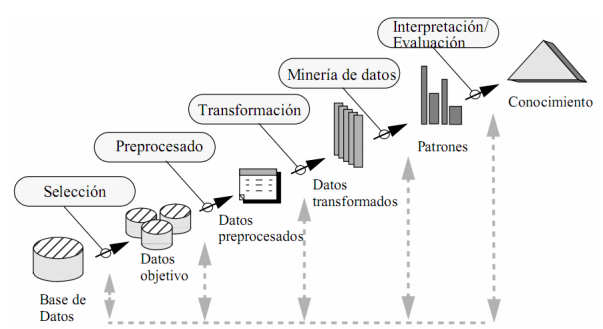
\includegraphics[width=1 \textwidth]{etapaskdd.png}
\caption{Etapas en el proceso de KDD}
\label{etapaskdd}
\end{figure}

\paragraph{En el proceso de KDD podemos distinguir una serie de etapas, como se puede observar en la Figura \ref{etapaskdd}, las cuales describimos a continuaci\'on: }

\begin{itemize}

\item \textbf{Selecci\'on:} En esta etapa, el objetivo es escoger una fuente o conjunto de fuentes de datos como entrada. La selecci\'on de las fuentes se da a partir del an\'alisis previo del problema, de tal manera que los datos escogidos sean representativos del problema y resulten \'utiles para descubrir conocimiento. Adem\'as, se pueden generar nuevos repositorios de datos a partir del conjunto de datos seleccionado. La recolecci\'on, descripci\'on y exploraci\'on de datos son tareas comunes en esta fase del proceso.
\item \textbf{Preprocesamiento:} Esta etapa involucra operaciones de limpieza y preprocesamiento de los datos, as\'i como tambi\'en de integraci\'on de diferentes fuentes de datos. Algunas tareas comunes que efect\'uan en esta etapa son la selecci\'on de columnas para el an\'alisis de datos, la limpieza de los datos con ``ruido'', eliminaci\'on de registros repetidos y la definici\'on de acciones sobre los campos con registros nulos.
\item \textbf{Transformaci\'on:} La transformaci\'on de datos se efect\'ua con el objetivo de conseguir una caracterizaci\'on o representaci\'on de los datos, acorde a los objetivos planteados y, si es posible, reducir la cantidad de variables o atributos considerados, buscando un buen desempe\~no en las siguientes fases del proceso. Algunas tareas comunes en esta etapa son la discretizaci\'on de valores, agrupaciones por tipos y la reducci\'on de variables.
\item \textbf{Extracci\'on de Patrones:} En esta etapa se llevan a cabo trabajos de decisi\'on sobre los modelos y par\'ametros adecuados para obtener resultados coherentes y esperados sobre los datos, mapeando dichos modelos con las tareas adecuadas de miner\'ia para cada criterio u objetivo definido en el modelado. Las tareas comunes en esta fase del proceso son la clasificaci\'on, agrupaci\'on, asociaci\'on, visualizaci\'on y sumarizaci\'on de elementos, adem\'as de la detecci\'on de desv\'ios, estimaci\'on de valores, an\'alisis de relacionamiento, entre otras.
\item \textbf{Interpretaci\'on y Evaluaci\'on:} De acuerdo a los datos obtenidos, este paso primariamente implica una retroalimentaci\'on de las etapas previas con el fin de corregir errores o mejorar ciertos procedimientos. Adem\'as se realiza una visualizaci\'on sobre los patrones y modelos obtenidos de manera a comprender dichos resultados y extraer conocimientos. Durante las acciones de comprensi\'on y descubrimiento de conocimiento, se pueden presentar casos en los cuales los resultados generen conflictos con algunos conocimientos previos, por tanto la resoluci\'on de dichos inconvenientes puede implicar la modificaci\'on o actualizaci\'on de ciertos par\'ametros aplicados en pasos anteriores.

\end{itemize}


\section{Preprocesamiento de entradas}
\paragraph{Este paso se efect\'ua previamente al de la estrategia de categorizaci\'on seleccionada, con el objetivo de limitar y refinar los espacios de b\'usqueda. En esta etapa del proceso se define cu\'ales entradas son relevantes y la disposici\'on m\'as eficiente en la que pueden ser introducidas al proceso de clasificaci\'on. Algunas t\'ecnicas de preprocesamiento son las siguientes:}

\begin{itemize}

\item \textbf{Utilizaci\'on de n-gramas:} Los datos pueden ser introducidos en forma de n-gramas. Un n-grama consiste en una subsecuencia de n-elementos de una secuencia dada. En el estudio del lenguaje natural, se pueden introducir elementos de distinta granularidad, como letras, s\'ilabas o palabras. Sin embargo, en el an\'alisis de sentimientos, generalmente se utilizan las palabras. El caso base para la disposici\'on de los datos es la utilizaci\'on de las palabras como unigramas (subsecuencias de un elemento). Otra variante muy utilizada y que es objeto de varios experimentos con resultados positivos, es la introducci\'on de bigramas (subsecuencias de dos palabras) con el objetivo de aumentar la precisi\'on en la determinaci\'on de la polaridad de los textos, partiendo de la idea que con ellas se puede lograr una mejor evaluaci\'on de intensificadores, negadores y otros fen\'omenos gramaticales; por ejemplo, ``muy bueno'', ``no apto'' son bigramas significativos.

\item \textbf{Eliminaci\'on de stopwords:} Las \textit{stopwords} son un conjunto de palabras de uso muy frecuente y que son omitidas en el proceso de b\'usqueda, pues no representan entradas significativas (ru\'ido) para el an\'alisis pertinente; en este caso, cargas de polaridad. Varias de ellas son propias de la gram\'atica, como art\'iculos, nombres, preposiciones y otras categor\'ias l\'exicas; algunos ejemplos son: ``ac\'a'', ``ah\'i'', ``alg\'un'', ``del'', ``en'', entre otras. Otras palabras no significativas para el an\'alisis de sentimientos pueden ser aquellas relativas al dominio, pues son utilizadas de manera muy frecuente y tampoco implican orientaci\'on a alguna polaridad determinada; por ejemplo, en una cr\'itica de cine, estas palabras podr\'ian ser ``actor'', ``actuaci\'on'', ``sonido'', entre otras.

\item \textbf{Stemming:} El m\'etodo de \textit{stemming} consiste en obtener la ra\'iz sem\'antica de cada palabra con el objetivo de asociar las palabras con dicha ra\'iz. Con esto se logra reducir las formas derivadas de las palabras a su forma base. Por ejemplo, la ra\'iz del verbo ``aprender'' es ``aprend'', con lo que se logra asociar las conjugaciones de dicho verbo como ``aprende'', ``aprendo'', ``aprendiendo'', etc.

\item \textbf{Lematizaci\'on} La lematizaci\'on es similar al m\'etodo de \textit{stemming}, a diferencia de que \'este toma como ra\'iz de las palabras un subconjunto de letras de la misma; mientras que en el proceso de lematizaci\'on, se busca hallar el lema de una palabra, es decir su forma gen\'erica o como la encontrar\'iamos en un diccionario. Por ejemplo, mediante lematizaci\'on se puede lograr reducir la forma ``hice'' a su lema ``hacer'', mientras que esto no ser\'ia posible mediante \textit{stemming}.

\item \textbf{An\'alisis de estructuras gramaticales:} Llamada tambi\'en POS (por sus siglas en ingl\'es, \textit{``part-of-speech''}). Consiste en el etiquetado de las palabras seg\'un su categor\'ia gramatical, debido a que algunas de ellas son indicadoras m\'as relevantes de opini\'on. Ciertas categor\'ias como por ejemplo, los adjetivos o los adverbios, son m\'as descriptivas para detectar polaridad en una oraci\'on que los sustantivos, los verbos o los art\'iculos. Algunas aplicaciones de esta t\'ecnica son la asignaci\'on de pesos a las palabras por categor\'ia o bien la utilizaci\'on de las etiquetas mismas como atributos para un conjunto de entrenamiento.

%\paragraph{POS Tagging, an\'alisis sint\'actico de dependencias, etc}

\end{itemize}



\section{Estrategias basadas en l\'exicos}
\paragraph{En cualquier lenguaje, existen palabras com\'unmente utilizadas para expresar opini\'on o ``sentimiento'' con una orientaci\'on determinada respecto a una entidad en particular. Dicha orientaci\'on puede ser positiva o negativa; por ejemplo: ``bueno'', ``genial'' y ``espectacular'' son entradas positivas; mientras que ``malo'', ``p\'esimo'' y ``horrible'' son entradas negativas. Estas palabras, denominadas \textit{sentiment words} (SW, por sus siglas en ingl\'es) en conjunto conforman un l\'exico de sentimientos u opiniones. Para conformar dicho l\'exico, pueden ser tomados como fuentes distintos textos escritos, cuyos contenidos traten de evaluar o expresar opini\'on sobre alguna entidad, como por ejemplo cr\'iticas, libros, recetas, p\'aginas Web, entre otros.} 
\paragraph{Las SW podemos clasificar en palabras descriptivas y comparativas. Las palabras descriptivas expresan calificaci\'on sobre una entidad, tales como las citadas en el p\'arrafo anterior; mientras que las palabras comparativas establecen confrontaci\'on entre dos entidades, generando opiniones superlativas. Por ejemplo, en la oraci\'on ``El producto A es mejor que el producto B'' no se establece calificaci\'on positiva ni negativa para alguno de los productos, sino que solamente en comparaci\'on al producto B, el A es mejor. Esto no implica que ``mejor'' sea exclusivamente una SW comparativa para cualquier oraci\'on, sino que cumple tal funci\'on en el contexto dado.}
\paragraph{En algunos l\'exicos, la orientaci\'on sem\'antica de las palabras es cuantificada generalmente por valores num\'ericos, que luego son introducidos en una funci\'on de puntuaci\'on, para determinar la polaridad de una opini\'on acerca de una entidad determinada. Dicha funci\'on var\'ia seg\'un el an\'alisis de distintos autores; as\'i como los criterios de cuantificaci\'on de las orientaciones sem\'anticas. En algunos trabajos, se limitan a asignar signos positivos y negativos (+1 y -1) a las palabras (Ding y otros, 2008); mientras que en otros, se emplea un intervalo m\'as amplio para obtener un mejor balance de la suma final de polaridades, como (Taboada y otros, 2011) que utilizan un intervalo de puntuaci\'on de -5 a +5. Estas puntuaciones, as\'i como las funciones definidas para el c\'alculo de polaridad, pueden influir en la precisi\'on de resultados logrados.}
\paragraph{En (Liu, 2012) se identifican tres tipos de estrategia para compilar SW que conformen un l\'exico: la generaci\'on manual, la generaci\'on basada en un diccionario y la generaci\'on basada en un corpus.}

\subsection{L\'exico generado manualmente}
\paragraph{Seguir esta estrategia implica un costo muy alto de trabajo y de tiempo, por tanto generalmente no es utilizada de manera exclusiva. Tiene su utilidad en combinaci\'on con estrategias automatizadas mediante tareas tales como una verificaci\'on final de palabras, puesto que con los m\'etodos automatizados se pueden generar errores.}

\subsection{L\'exico basado en un diccionario}
\paragraph{La construcci\'on de un diccionario implica un listado de sin\'onimos y ant\'onimos para cada palabra. Un m\'etodo sencillo de generaci\'on es utilizar como semillas algunas SW, a partir de las cuales se pueden encontrar las dem\'as palabras del diccionario a partir de los sin\'onimos y ant\'onimos de las semillas. A medida que dichos sin\'onimos son agregados como nuevas palabras semilla, el diccionario va creciendo sucesivamente. Algunos trabajos que se ocupan de la generaci\'on de un diccionario son (Hu y Liu, 2004) y (Kim y Hovy, 2004).}
\paragraph{La ventaja de utilizar un diccionario es que se puede encontrar f\'acil y r\'apidamente un gran n\'umero de SW con sus orientaciones sem\'anticas. A pesar de que la lista resultante puede incluir varios errores, es posible efectuar una verificaci\'on manual de limpieza para refinar el diccionario. Por otro lado, la principal desventaja es que la lista de palabras generadas en un diccionario son de prop\'osito muy general (no orientadas al dominio de aplicaci\'on) y dependientes del contexto. Esta dificultad puede tratada mediante la generaci\'on de un corpus.}

\subsection{L\'exico basado en un corpus}
\paragraph{Esta estrategia fue mayormente aplicada frente a dos escenarios:}
\begin{enumerate}
\item Dado un listado base de SW conocidas, de prop\'osito general, se descubren nuevas SW con sus orientaciones para un determinado dominio.
\item Adaptar un l\'exico de prop\'osito general a uno nuevo utilizando un corpus para aplicaciones de an\'alisis de sentimientos en el dominio.
\end{enumerate}
\paragraph{Construir un l\'exico de sentimientos para un dominio espec\'ifico puede no ser suficiente puesto que en el mismo dominio, una misma palabra puede ser positiva en un contexto, pero negativo en otro. Esta estrategia tambi\'en puede ser utilizada para construir un l\'exico de prop\'osito general en el caso que se encuentre disponible un corpus muy grande y diverso, pero para tal prop\'osito es m\'as efectiva la elaboraci\'on de un diccionario, puesto que el mismo ya est\'a compuesto por todas las palabras. Algunos trabajos que tratan la generaci\'on de un corpus son (Turney, 2002) y (Ding y otros, 2008). }

\subsection{Procesamiento de Lenguaje Natural}
\paragraph{Para extraer las opiniones o sentimientos (informaci\'on) a partir de un texto, el an\'alisis del mismo debe ser tratado como un problema de PLN. Como tal, debe considerar todos los aspectos de ella, como por ejemplo la desambiguaci\'on de palabras, las negaciones, intensificaciones, decrementaciones, entre otros.}
\paragraph{El problema espec\'ifico de extracci\'on de opiniones, es un problema de PLN restringido puesto que no es necesario entender completamente la sem\'antica de cada oraci\'on o documento, mas debe interpretar \'unicamente ciertos aspectos de ellos, como los sentimientos positivos o negativos y las entidades o t\'opicos a los que se refieren. De todas maneras, existen tambi\'en otros problemas a\'un no resueltos de PLN que agregan ciertas dificultades al proceso de an\'alisis. A continuaci\'on, describimos algunos t\'opicos que representan tanto aspectos comunes como dificultades que son tratadas en los problemas de PLN.}

\begin{itemize}

\item \textbf{Desambiguaci\'on de palabras:} Es un aspecto a llevar en cuenta, puesto que en el lenguaje de entrada pueden existir varias palabras que presentan polisemia, es decir cuando una  misma palabra representa diversos significados o acepciones. Esto conduce a que parte del problema considerado es identificar 	el sentido de la palabra dentro de una determinada oraci\'on o documento. Por ejemplo, la palabra ``vaya'' podr\'ia representar un verbo conjugado en presente subjuntivo, en modo imperativo, o incluso una interjecci\'on que denota admiraci\'on o asombro. La diferenciaci\'on de dichos significados es una capacidad humana sencilla, pero debe poder reproducirse adem\'as en los algoritmos de interpretaci\'on que sean desarrollados.
\item \textbf{Negaci\'on:} Es un elemento ling\"u\'istico que, como lo dice su nombre, se utiliza para negar una oraci\'on entera o alguna idea contenida en ella, mediante la utilizaci\'on de adverbios de negaci\'on. Tales adverbios pueden ser utilizados en distintos \'ordenes para referirse a la idea negada, es decir pueden aparecer antes, en medio o despu\'es de ellas. Algunos de estos adverbios de negaci\'on son ``no'', ``nunca'', ``jam\'as'', ``tampoco'', ``nada'' y ``negativamente''.
\item \textbf{Intensificaci\'on y Atenuaci\'on:} Consisten en la utilizaci\'on de ciertos adverbios como recursos ling\"u\'isticos para aumentar o disminuir la intensidad de alguna idea transmitida.  Algunos intensificadores de ejemplo son ``muy'', ``mucho'', ``demasiado'' y ``sobremanera'',  mientras que adverbios como ``poco'', ``menos'', ``solamente'', ``apenas'', ``justo'' son atenuadores.
\item \textbf{Palabras dependientes del contexto:} Son aquellas que no pueden ser definidas como orientadas positivamente o negativamente, sin conocer el dominio del tema que se est\'e abordando. Una palabra puede ser utilizada para referirse positivamente hacia una entidad en un determinado dominio; pero a la vez dicha palabra puede tener una implicancia negativa en un dominio diferente.
Por ejemplo, el adjetivo ``peque\~no'' puede ser visto como positivo refiri\'endose al tama\~no de un tel\'efono celular; o bien como negativo si es referido al tama\~no de una porci\'on de comida servida en un comedor.
\item \textbf{M\'ultiples orientaciones sem\'anticas:} Se presentan cuando se efect\'ua el an\'alisis de un texto que puede estar compuesto por varias oraciones, o bien varias ideas y \'estas pueden tener polaridades diferentes. La entidad a la que se est\'a refiriendo el texto puede ser la misma, pero distintas oraciones pueden referirse a diferentes caracter\'isticas de ella.  Por ejemplo, en la siguiente referencia a una c\'amara fotogr\'afica: ``La calidad de las im\'agenes es muy buena, pero la duraci\'on de la bater\'ia es muy corta.'', la opini\'on acerca de la caracter\'istica de calidad de las im\'agenes es positiva, mientras que la duraci\'on de la bater\'ia es vista negativamente. Ambas aparecen en una misma oraci\'on y adem\'as se refieren a la misma entidad, la c\'amara fotogr\'afica.
\item \textbf{Sarcasmo:} Es una figura que genera dificultades pues cuando se encuentra presente en una oraci\'on, pretende dar a entender lo contrario a lo que las palabras expresan. Es decir, se pueden encontrar varias palabras con orientaci\'on positiva, con la intenci\'on de manifestar negativismo de manera evidente, o viceversa.

\end{itemize}



\section{Estrategias basadas en aprendizaje de m\'aquina}
\paragraph{La estrategia basada en aprendizaje de m\'aquina, tambi\'en referida como estad\'istica o clasificadora de textos, consiste en entrenar un clasificador para categorizar elementos de entrada dentro de una clase perteneciente a un conjunto definido de clases; por ejemplo, de sentimientos positivos, negativos o neutrales. El objetivo es generalizar comportamientos a trav\'es de informaci\'on previamente recolectada, denominada conjunto de entrenamiento, en forma de ejemplos, que luego puedan ser utilizados para evaluar un texto en funci\'on a sus similaridades.}
\paragraph{En t\'erminos generales un conjunto de entrenamiento, llamado en ingl\'es \textit{training set}, es un conjunto de datos que se utiliza para realizar pruebas iniciales sobre un modelo conceptual esperando conseguir una descripci\'on comprensible de dicho modelo y a partir del mismo, la generaci\'on de conocimiento.}
\paragraph{Podemos identificar dos tipos de aprendizaje en esta estrategia: supervisado y no supervisado.}
\paragraph{En un m\'etodo de aprendizaje supervisado, se produce una funci\'on de correspondencia entre las entradas y salidas deseadas del sistema; como por ejemplo clasificar las palabras seg\'un su categor\'ia l\'exica (verbos, sustantivos, adjetivos, etc), categor\'ia funcional (determinantes, cuantificadores, pronombres, etc) o su polaridad (positivas, negativas, neutras, etc), por lo que se necesita una base de conocimiento previamente elaborada, compuesta por ejemplos de etiquetados anteriores.}
\paragraph{Los m\'etodos de aprendizaje no supervisado se llevan a cabo sobre conjuntos de ejemplos conformados \'unicamente por entradas al sistema; sin etiquetado de categor\'ias, a diferencia de los m\'etodos supervisados; por lo que el sistema debe tener capacidad de reconocimiento de patrones para etiquetar nuevas entradas. }
\paragraph{Algunos clasificadores de aprendizaje de m\'aquina son \textit{Na\"ive Bayes} (NB), \textit{Maximum Entropy} (ME) y \textit{Support Vector Machines} (SVM). En las siguientes subseccciones, definimos cada uno de ellos, utilizando el siguiente conjunto de variables:}

\begin{itemize}
\item Un corpus de texto $C$, compuesto por una serie de documentos. La cantidad de documentos es irrelevante y cada uno de ellos es denominado $d$. 
\item Un conjunto de clases $\{c_{1},c_{2},\ldots,c_{n}\}$ definido.
\item Un conjunto de palabras que componen el corpus $C$. Todas las palabras $w$ que componen $C$ representan los atributos del conjunto de entrenamiento.
\end{itemize}
\paragraph{El objetivo es determinar a qu\'e clase $c$ pertenece cada documento $d$.}

\subsection{Na\"ive Bayes}
\paragraph{El algoritmo basado en el teorema de Bayes, aplicado al an\'alisis de textos, consiste en clasificar cada palabra de acuerdo a la probabilidad de que pertenezca a un determinado grupo. Tales agrupaciones pueden estar determinadas por categor\'ias gramaticales o por polaridad. 
La clasificaci\'on por etiquetas gramaticales (\textit{POS tagging}) permite, por ejemplo, establecer la probabilidad de que la palabra siguiente a un sustantivo sea un verbo; con el objetivo de determinar qu\'e influencia tiene una palabra en la polaridad de un texto. En este contexto, un adjetivo es m\'as descriptivo que un sustantivo para la inferencia del sentimiento transmitido en un texto.
La asociaci\'on por polaridad, en cambio relaciona las palabras que componen una oraci\'on con el sentimiento que ellas en conjunto transmiten. Es decir, las palabras utilizadas en una oraci\'on considerada positiva son, con mayor probabilidad, palabras con asociaci\'on positiva para cualquier otra oraci\'on.}
\paragraph{El clasificador \textit{Na\"ive Bayes} deriva del teorema de la probabilidad condicional de dos eventos aleatorios $A$ y $B$ enunciado por Thomas Bayes, donde ``la probabilidad del evento $A$ dado $B$'' est\'a expresado por la siguiente f\'ormula:}
$$P(A \, | \, B) \, = \, {P(A) \, P(B \, | \, A) \over P(B)},$$
\paragraph{Llevando dicho teorema al problema de la clasificaci\'on de textos y utilizando el conjunto de variables antes definido, el primer paso consiste en estimar la probabilidad $P(c)$ de cada clase $c$, dividiendo el n\'umero de palabras presentes en los documentos etiquetados en $c$ entre la cantidad total de palabras en el corpus $C$. Luego, la distribuci\'on de probabilidad $P(w \, | \, c)$ para todas las palabras por cada clase $c$ est\'a dada por la divisi\'on de la cantidad de ocurrencias de $w$ en los documentos etiquetados en $c$ entre la cantidad de palabras en $c$.}
\paragraph{De esta manera, podremos asignar un valor num\'erico a un documento para cada una de las clases, para luego asociarlo a una de ellas. Dicho valor est\'a dado por:}
$$ score(d \, | \, c) \, = \, P(c) \, * \, \prod_{i=1}^n \, P(w_{i} \, | \, c) $$

\paragraph{Luego, la estimaci\'on del modelo ser\'a de aquella clase cuyo valor de $score$ haya resultado mayor que el valor obtenido para las dem\'as clases.}
\paragraph{La dificultad en la aplicaci\'on de este algoritmo es que est\'a cimentado en la hip\'otesis de que las variables evaluadas son independientes entre s\'i (visto en la multiplicaci\'on de los valores de $P(w_{i} \, | \, c)$ en la definici\'on de $score$); y como la gram\'atica es por el contrario, dependiente del contexto, muchas entradas son clasificadas err\'oneamente, originando los fen\'omenos conocidos como ``falsos positivos'' o ``falsos negativos'' si tratamos la polaridad. Sin embargo, los resultados pueden ser a\'un muy positivos con la determinaci\'on de un buen conjunto de entrenamiento.}

\subsection{Maximum Entropy}
\paragraph{El clasificador por entrop\'ia m\'axima trata de generar informaci\'on reduciendo el sesgo al m\'inimo posible. El principio fundamental del algoritmo es que son preferidas las distribuciones uniformes que satisfacen adem\'as todas las restricciones del problema (Nigam y otros, 1999). Dichas restricciones que caracterizan al modelo, son derivadas de los datos etiquetados del conjunto de entrenamiento.}
\paragraph{El algoritmo trata de identificar las caracter\'isticas que definen una clase, definiendo un modelo que englobe las reglas que puedan ser inferidas del conjunto de entrenamiento. Luego, estima un valor esperado para cada una de las clases definidas, de manera a tratarlos como restricciones en el modelo de distribuci\'on (Lee y Renganathan, 2011).}
\paragraph{A diferencia del algoritmo de \textit{Na\"ive Bayes}, no asume la independencia entre variables. En cambio, el modelo busca mediante las restricciones mencionadas, maximizar la adherencia entre atributos en relaci\'on a alguna clase, de tal manera que una nueva entrada ser\'a categorizada dentro una clase cuanto menos caracter\'isticas extr\'insecas a su definici\'on contenga.}
\paragraph{Nigam y otros (1999) definen la probabilidad $P(c \, | \, d)$ de cada clase de la siguiente manera:}
$$ P(c \, | \, d) \, = \, {1 \over Z(d)} \, exp \, 
\left(
\sum_{i} \lambda_{i}F_{i}(d,c)
\right) ,$$
\paragraph{Con la siguiente definici\'on de par\'ametros:}
\begin{itemize}
\item Cada $F_{i}(d,c)$ es un atributo
\item $\lambda_{i}$ es el par\'ametro a ser estimado. Es un indicador de peso; es decir, un valor mayor indica que $F_{i}$ es un indicador m\'as relevante para la clase $c$.
\item $Z(d)$ es una funci\'on de normalizaci\'on para definir una probabilidad apropiada, dada por la siguiente expresi\'on:
$$
Z(d) = \sum_{c} \, exp \, \left( \sum_{i} \lambda_{i}F_{i}(d,c)  \right)
$$
\end{itemize}

\paragraph{La b\'usqueda de $\lambda_{i}$ se realiza por medio de algoritmos de b\'usqueda iterativa definidos seg\'un el modelo, como por ejemplo el m\'etodo de \textit{Hill Climbing} o el de temple simulado.}

\paragraph{Las dificultades que pueden presentarse con el m\'etodo de entrop\'ia m\'axima son la facilidad con la que se presentan casos de \textit{overfitting} (sobreentrenamiento del algoritmo con los datos de entrada dados, que produce p\'erdida de generalizaci\'on para datos nuevos) y el tiempo que pueda emplearse en la determinaci\'on de los pesos puesto que las iteraciones para calcularlos pueden llegar a ser infinitas.}

\subsection{Support Vector Machines}
\paragraph{La t\'ecnica de clasificaci\'on por \textit{Support Vector Machines} efect\'ua la separaci\'on de puntos un espacio $N$-dimensional utilizando un hiperplano $(N-1)$-dimensional, a diferencia de las t\'ecnicas de Bayes y entrop\'ia m\'axima, que utilizan medidas probabil\'isticas para clasificar los puntos. Dado un conjunto de entrenamiento, el clasificador por SVM busca encontrar un hiperplano con el mayor margen posible, de manera que cada punto del conjunto de entrenamiento sea clasificado correctamente y que el hiperplano se encuentre a la m\'axima distancia posible de sus puntos m\'as cercanos. La clasificaci\'on de las instancias de entrenamiento consiste en determinar a qu\'e lado del hiperplano caen ellas. En la pr\'actica, es posible que no se encuentre un hiperplano que separe los grupos perfectamente, por lo que los puntos pueden hallarse dentro del margen o del lado incorrecto del hiperplano.}
\paragraph{Si representamos el hiperplano buscado por el vector $\vec{w}$, la b\'usqueda corresponde a un problema de optimizaci\'on con restricciones, siendo $c_{j} \, \in \, \{1,-1\}$ (positiva y negativa) la clase correcta del texto $d_{j}$, la soluci\'on puede ser escrita como:}
$$ \vec{w} \, := \, \sum_{j} \alpha_{j}c_{j}\vec{d_{j}}, \quad \alpha_{j} \, \geq \, 0, $$
\paragraph{donde las $\alpha_{j}$ son obtenidas por resoluci\'on de un problema de optimizaci\'on. Los vectores $\vec{d_{j}}$, tal que $\alpha_{j}$ es mayor que cero, son llamados vectores de soporte, dado que son los \'unicos que contribuyen al hiperplano $\vec{w}$.}
\paragraph{Ha sido demostrado varias veces que este m\'etodo es altamente efectivo para la categorizaci\'on de textos, obteniendo generalmente mejores resultados que la t\'ecnica de Bayes (Joachims, 1998; Pang y otros, 2002; Kennedy e Inkpen, 2006).}


\section{M\'etricas de evaluaci\'on}
\paragraph{La evaluaci\'on de la clasificaci\'on se efect\'ua primariamente con el objetivo de comparar el desempe\~no de distintos sistemas o m\'etodos entre s\'i. La relevancia y utilidad de los resultados obtenidos prevalecen sobre los tiempos y espacios de respuesta cuando evaluamos una estrategia de an\'alisis de textos. No existe un \'unico criterio que permita determinar que un m\'etodo es mejor que otro; por ello, existen diversas m\'etricas para medir la efectividad de la informaci\'on obtenida del an\'alisis.}
\paragraph{Las m\'etricas que presentamos en esta secci\'on est\'an basadas en la matriz de confusi\'on o de clasificaci\'on. Dicha matriz contrasta la estimaci\'on del modelo clasificador para un elemento dado, con la clase real asociada a dicho elemento.}
\paragraph{Dado un conjunto de datos $E$, donde cada elemento $e$ puede ser representado como un vector $< e_1, e_2, \dots, e_n >$ de $n$ atributos, y un conjunto de clases $C$; cada vector $e \in E$ tiene una clase $c \in C$ asociada. La clasificaci\'on consiste en asignar una clase $c \in C$ para cada elemento $e \in E$, y el objetivo es cuantificar la efectividad de dichas asignaciones. Para dicho efecto, las filas de la matriz de confusi\'on representan las clases reales a la que pertenecen cada uno de los elementos y las columnas representan a la predicci\'on del modelo clasificador, como se observa en el Cuadro \ref{matrizconfusion}.}

\begin{table}[htb] 
\centering

$
\begin{array}{|c|c|c|c|}
      \hline
         				& \mathbf{Clase_1}	& \mathbf{Clase_2}	& \mathbf{Clase_n}	\\
      \hline
      \mathbf{Clase_1}  & V	Clase_1	& F Clase_2	& F Clase_n	\\
      \hline
      \mathbf{Clase_2} 	& F Clase_2 & V Clase_2 & F Clase_n	\\
      \hline
      \mathbf{Clase_n}	& F Clase_n	& F	Clase_2	& V Clase_n	\\
      \hline
\end{array}
$
\caption{Matriz de confusi\'on o de clasificaci\'on}
\label{matrizconfusion}
\end{table}

\paragraph{Referenciando los sub\'indices de filas y columnas como $[i,j]$, una entrada Verdadera representa un acierto, es decir si el clasificador ha determinado que un elemento $e$ pertenece a la $Clase_j$ y dicho elemento efectivamente est\'a asociado a la $Clase_j$; mientras que una entrada Falsa representa un error de clasificaci\'on, es decir que el elemento $e$ no pertenec\'ia efectivamente a la $Clase_j$.} 
\paragraph{Definimos a continuaci\'on algunas m\'etricas de evaluaci\'on, en cuyas definiciones referenciamos a los aciertos y errores con el sub\'indice de la fila $i$ a la que pertenecen en la matriz de confusi\'on, como Verdadero de la $Clase_i$ o Falso de la $Clase_i$ :} 

\subsection{Precisi\'on}
\paragraph{La precisi\'on respecto a la $Clase_i$ indica el n\'umero de predicciones correctas sobre el total de predicciones de dicha clase. Es decir, indica la probabilidad de que un elemento $e$ pertenezca realmente a la $Clase_i$ dado que fue identificado como tal por el clasificador. Est\'a dado por la proporci\'on de verdaderos de la $Clase_i$ en relaci\'on a los totales identificados como de dicha clase: }
\paragraph{
$$ Precisi\acute{o}n = {V Clase_i \over V Clase_i + F Clase_i} $$ }
\subsection{Recall}
\paragraph{El \textit{recall} respecto a la $Clase_i$ indica el n\'umero de predicciones acertadas como $Clase_i$ sobre el total de elementos que realmente pertenecen a dicha clase. Es la probabilidad de que un elemento $e$ que pertenece realmente a la $Clase_i$ sea clasificado como tal. Est\'a dado por la raz\'on entre los verdaderos de la $Clase_i$, sobre los elementos reales de la $Clase_i$, en la matriz de confusi\'on dados por la suma de los verdaderos de la $Clase_i$ m\'as los falsos de las dem\'as clases.}
\paragraph{
$$ Recall = { V Clase_i \over V Clase_i + F Clase_j } \quad donde \quad j \in \lbrace 1,2,\dots,n \rbrace \quad con \quad j \ne i $$ }
\subsection{Medida-F}
\paragraph{Relaciona las medidas de precisi\'on y \textit{recall} mediante una media con el mismo peso para ambas. Es conocida tambi\'en como $F_1$ por la uniformidad de los pesos.}
\paragraph{
$$ Medida-F = {2 \, \times Precisi\acute{o}n \, \times \, Recall \over Precisi\acute{o}n \, + \, Recall}$$ }



\section{Propuestas similares}
\paragraph{En esta secci\'on, describimos algunas propuestas publicadas recientemente, con el fin de conocer los \'ultimos enfoques presentados que fueron utilizados efectivamente para an\'alisis de sentimientos. Seleccionamos preferentemente trabajos con similitudes tales como el idioma abordado (espa\~nol o enfoques multiling\"ues), las fuentes de datos (mediadores de redes sociales) o las estrategias utilizadas (mediante l\'exicos o aprendizaje de m\'aquina).}

\paragraph{Moreno-Ortiz y P\'erez Hern\'andez (2013) presentan una propuesta basada en un l\'exico para categorizar textos cortos, al principio en cuatro categor\'ias de polaridad (positivos, negativos, neutros o sin polaridad) y luego agregando dos categor\'ias m\'as (muy positivos y muy negativos). El c\'alculo de polaridad est\'a centrado principalmente en dos valores num\'ericos denominados \textit{Global Sentiment Value} (GSV) y \textit{Affect Intensity} (AI); el primero, es un valor dentro de la escala de 0 a 10 asignado a sentimientos de acuerdo a una entrada de texto a partir del AI, el cual modula el GSV para reflejar el porcentaje de palabras con cierta carga de sentimientos. El AI no es un contador de palabras por polaridad, sino que de segmentos de texto que correspondan a unidades l\'exicas, definido como el porcentaje de segmentos que presentan determinada carga de polaridad, representando un paso intermedio para el ajuste de los l\'imites superior e inferior de las valencias relacionadas con el grado de sentimientos. Finalmente, concluyen que los valores de GSV se ven fuertemente afectados por la escasez de segmentos l\'exicos en los mensajes de Twitter; que la tendencia de la herramienta utilizada es la asignaci\'on de clasificaciones promedio, reflejada en la baja precisi\'on para las dos \'ultimas categor\'ias agregadas como ``extremos'' y adem\'as, que no es recomendable la diferenciaci\'on entre la categor\'ia de neutro con la de ausencia de polaridad.}

\paragraph{Vilares, Alonso y G\'omez-Rodr\'iguez (2013) presentan una propuesta basada en un l\'exico complementada con an\'alisis sint\'actico de dependencias, para tratar las construcciones ling\"u\'isticas e identificar los elementos implicados en las oraciones. El preprocesamiento, fundamental para el posterior an\'alisis sint\'actico, implica la unificaci\'on de expresiones compuestas que act\'uan como una sola unidad de significado, la normalizaci\'on de signos de puntuaci\'on y la segmentaci\'on del texto en oraciones, adem\'as de la separaci\'on de ellas en \textit{tokens} de palabras y signos de puntuaci\'on. El \'arbol de dependencias creado permite identificar relaciones binarias entre los elementos de una oraci\'on, en el cual cada v\'inculo constituye una funci\'on sint\'actica que relaciona dos t\'erminos. En cuanto al an\'alisis sem\'antico, la propuesta se basa en el diccionario de polaridad compuesto de adjetivos, sustantivos, verbos, adverbios e intensificadores propuesto por (Brooke, Tofiloski y Taboada, 2009), con la diferencia de que utilizan el \'arbol de dependencias para determinar cu\'al segmento de una oraci\'on se ve afectado por la modificaci\'on de los intensificadores, por la negaci\'on y las oraciones adversativas. En este trabajo, no se tratan los problemas de las palabras orientadas al dominio ni las figuras literarias tales como la iron\'ia o el sarcasmo. Concluyen que las t\'ecnicas de an\'alisis de dependencias resultan \'utiles para identificar de manera fiable el alcance de la negaci\'on en las oraciones y adem\'as proponen futuras adecuaciones para expresiones desiderativas as\'i como para el tratamiento de textos cortos.}

\paragraph{Bautin, Skiena y Vijayarenu (2008) presentan una propuesta multiling\"ue, mediante traducci\'on por m\'aquina con el fin de contrastar diferentes lenguajes de corpus paralelos. El an\'alisis fue hecho sobre escritos formales en nueve lenguajes, y adem\'as un corpus paralelo de cinco idiomas. Concluyen finalmente que la t\'ecnica de normalizaci\'on propuesta permite que la comparaci\'on de categorizaci\'on por polaridad en idiomas diferentes sea posible y que los errores de traducci\'on no son significativos, haciendo viables las comparaciones interculturales para an\'alisis de sentimientos.}

\paragraph{Una estrategia de co-entrenamiento es la propuesta de Wan (2009) para crear un l\'exico en Mandar\'in a partir de uno en Ingl\'es. Un conjunto de documentos de cada idioma, elaborados a trav\'es de traducci\'on por m\'aquina, son utilizados para evaluar el clasificador. Para estimar la polaridad de un documento en particular, deber\'ia ser clasificado correctamente tanto en Ingl\'es como en Mandar\'in. Los resultados demuestran que la propuesta presentada es muy efectiva para el tratamiento de diversos lenguajes.}

\paragraph{Boey y Moens (2008) presentan una estrategia de aprendizaje de m\'aquina que eval\'ua modelos mediante una arquitectura en cascada por capas, contando como fuente con un n\'umero limitado de entradas etiquetadas y en las cuales los textos no son escrituras formales. La propuesta consiste en tres capas de evaluaci\'on, cada una con diferente precisi\'on y velocidad en la computaci\'on de los resultados. Los idiomas tratados son el Ingl\'es, el Holand\'es y el Franc\'es. La clasificaci\'on en diferentes lenguajes es adem\'as tratada separadamente, de tal manera que puedan ser discutidas las diferencias entre los resultados obtenidos sobre cada uno de ellos. La conclusi\'on a la que arribaron es que el aprendizaje activo y continuo produce una notoria mejor\'ia sobre las muestras seleccionados aleatoriamente para el etiquetado, y adem\'as que el rendimiento obtenido fue mejor cuando aplicaron un filtro sobre las oraciones neutrales previa a la aplicaci\'on de los algoritmos de clasificaci\'on.}

\paragraph{} 

\section{Discusi\'on final del cap\'itulo}
\paragraph{En este cap\'itulo, presentamos los fundamentos te\'eoricos del an\'alisis de sentimientos, primeramente descripto de manera general como un proceso de descubrimiento de conocimiento, en el cual tras seleccionar, procesar y transformar los datos de entrada, buscamos extraer patrones para generar informaci\'on, que finalmente debe ser evaluada para cuantificar su utilidad. Luego, describimos las dos alternativas principales que existen para categorizar textos por polaridad; siendo uno de ellos basado en un l\'exico, es decir, vali\'endose de un diccionario o un corpus de entrada y teniendo en cuenta las reglas gramaticales del lenguaje de entrada; y por otro lado, la estrategia por aprendizaje de m\'aquina, que busca detectar patrones a trav\'es de un conjunto de entrenamiento generado previamente para permitir clasificar nuevas entradas dentro de un grupo de clases definidas.}
\paragraph{Describimos adem\'as algunas m\'etricas de evaluaci\'on que ser\'an utilizadas luego en  el problema propuesto, pues uno de los objetivos es comparar entre s\'i, el rendimiento obtenido tras la aplicaci\'on de las diferentes estrategias citadas. Sumarizamos finalmente, el estado del arte describiendo algunos trabajos con caracter\'isticas similares a las propuestas en este documento. En ellos, vemos que se utilizan los algoritmos ya presentados, que se tratan lenguajes diferentes en un mismo clasificador y que se da un tratamiento particular a los textos en formato corto e informal.}
\paragraph{En el siguiente cap\'itulo, describimos el problema a tratar, el modelado propuesto para resolverlo, en base a los fundamentos esbozados en este cap\'itulo y los objetivos de evaluaci\'on trazados.}

\chapter{Modelado del problema}\label{formulacion}

El ``jopara'', escrito y hablado en Paraguay, seg\'un Lustig (1996) ``en sentido estricto escapa a la condici\'on de una \textit{lengua}'' y es mejor descrito como una ``\textit{mezcla de lenguas} que como una \textit{lengua mezclada}''. Compuesto por el uso de palabras tanto del espa\~nol como del guaran\'i en una misma entidad de texto (documento, oraci\'on o incluso palabra), no se trata de un lenguaje oficial, ni tampoco de un dialecto por lo que no se disponen de reglas ni regulaciones formales expl\'icitas para la construcci\'on de oraciones. Este hecho representa la dificultad principal para la creaci\'on de un l\'exico as\'i como para el entrenamiento de un clasificador.
\newline

En el lenguaje natural utilizado entre las personas para comunicarse, se puede notar el uso frecuente del jopara, incluso en las redes sociales. Esto nos lleva considerar relevante su uso para el an\'alisis de sentimientos, particularmente porque las palabras originadas del guaran\'i son generalmente utilizadas para enfatizar sentimiento. Por ejemplo, en la oraci\'on \textit{``Kore! Ndoikoi ko aparato, encima que lo compr\'e reci\'en''}, las palabras ``kore'', ``ndoikoi'' y ``ko'' est\'an escritas en guaran\'i, y el resto de ellas en espa\~nol. Claramente, en esta oraci\'on, el indicador m\'as evidente de negatividad en esta oraci\'on es la interjecci\'on que la inicia.
\newline

En este cap\'itulo, presentamos el modelado propuesto para aplicar las t\'ecnicas de categorizaci\'on descriptas en el cap\'itulo anterior sobre el lenguaje abordado. Describimos algunos patrones de formaci\'on de palabras en el jopara, el formato de entrada de los textos en Twitter y establecemos algunas reglas de preprocesamiento para lograr una selecci\'on adecuada de atributos de entrada para los clasificadores.
\newline \newline

\section{Caso de estudio: Reacciones de clientes de una compa\~n\'ia de telecomunicaciones}

Con el fin de efectuar un an\'alisis que permita detectar la polaridad de los sentimientos en un escenario dado, tomamos en cuenta las opiniones expresadas por los usuarios de una compa\~n\'ia de telecomunicaciones que domina gran parte de dicho mercado, en un mediador de redes sociales de uso masivo. Twitter es una de las herramientas de interacci\'on m\'as populares entre los usuarios de Internet, y dado su formato libre y corto de mensajes adem\'as de su accesibilidad, recopilamos un corpus de 20.000 textos que representan interacciones de los usuarios con la compa\~n\'ia en cuesti\'on, es decir los mensajes que contengan una menci\'on de la cuenta de dicha compa\~n\'ia en la red de Twitter.
\newline

Presentamos entonces, el an\'alisis sobre un corpus compuesto por una variedad de lenguajes. Si observamos los contenidos compartidos por los usuarios en el corpus extra\'ido, notamos que las oraciones est\'an escritas no solamente en los lenguajes nativos oficiales de Paraguay sino que adem\'as en jopara, ingl\'es y portugu\'es. Por tanto, proponemos el tratamiento de dichos lenguajes en conjunto mediante la aplicaci\'on de los m\'etodos existentes de an\'alisis, centr\'andonos principalmente en la selecci\'on de atributos y la calibraci\'on de los par\'ametros de entrada para los algoritmos.
\newline

Previamente a la descripci\'on general del procedimiento seguido, describimos las caracter\'isticas del formato de los mensajes compartidos en Twitter (tuits).

\section{Caracterizaci\'on de mensajes en Twitter}

Los mensajes compartidos en Twitter poseen varias caracter\'isticas \'unicas, que los diferencian de los dem\'as corpus de datos citados previamente. (Go y otros, 2009) identifican cuatro de ellas:

\begin{itemize}
\item \textbf{Longitud m\'axima:} Cada publicaci\'on puede estar compuesta por una cantidad m\'axima de 140 caracteres, incluyendo signos de puntuaci\'on y s\'imbolos.
\item \textbf{Alta disponibilidad:} La API de Twitter permite obtener tuits libremente, a trav\'es de su funci\'on de b\'usqueda. Mediante esta funci\'on es posible recolectar una cantidad de tuits considerable para conformar los conjuntos de entrenamiento y de evaluaci\'on.
\item \textbf{Modelo del lenguaje:} Los mensajes de Twitter pueden ser generados desde diversos dispositivos, incluyendo los tel\'efonos celulares. Esto lleva a que los errores ortogr\'aficos y expresiones informales se hagan mucho m\'as frecuentes en comparaci\'on a otros dominios.
\item \textbf{Dominio:} Los tuits se refieren a diversos temas, lo cual es relevante puesto que un gran porcentaje de estudios pasados fueron centrados en un dominio espec\'ifico.
\end{itemize}

Existen adem\'as ciertas convenciones de lenguaje de los tuits:
\begin{itemize}
\item ``RT'' es un acr\'onimo de retuit, que se coloca delante de un mensaje para indicar que el mismo est\'a siendo repetido o compartido.
\item El caracter ``\#'' es utilizado para marcar, organizar y clasificar tuits por temas o categor\'ias.
\item El caracter ``@'' es empleado para referirse a una cuenta por su nombre de usuario.
\end{itemize}

Es frecuente adem\'as que los tuits vayan acompa\~nados de emoticones y v\'inculos de Web. La influencia de las caracter\'isticas de estos mensajes en nuestra propuesta es abordada en la siguiente secci\'on.

\section{Procedimiento general}\label{procedimiento}
El procedimiento seguido para generar los resultados desde los tuits recolectados inicialmente se muestra en la Figura \ref{overview}. Como se puede observar, en algunas etapas del mismo se producen ciertos productos intermedios significativos como el corpus, el l\'exico y el conjunto de entrenamiento antes de llegar a los resultados.
\newline

\begin{figure}[h]
\centering
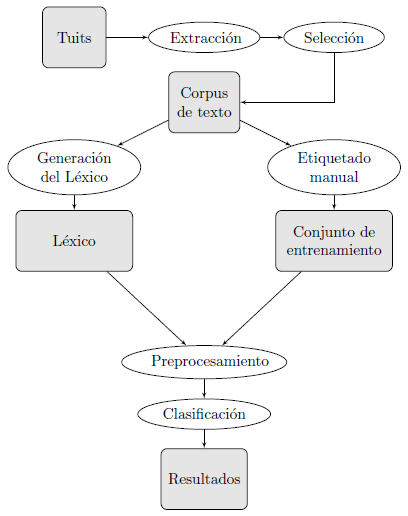
\includegraphics[width=0.7\textwidth]{overview.png}
\caption{Vista general del proceso seguido para obtener los resultados.}
\label{overview}
\end{figure}

Las etapas de las que se compone el proceso son las siguientes:
\begin{itemize}
\item \textbf{Extracci\'on:} Recolectamos inicialmente 20.000 tuits con alguna menci\'on a la compa\~n\'ia objeto. Esto fue logrado mediante el uso de la API de Twitter \footnote{https://dev.twitter.com/docs/api (Version 1.1)}.  Cada tuit retornado en una consulta contiene varios atributos relativos a las interacciones entre usuarios, de los cuales utilizamos \'unicamente el cuerpo de texto, como objeto de estudio, y el n\'umero identificador de cada uno, para evitar duplicaciones; en tanto, los dem\'as atributos son irrelevantes para los objetivos trazados en este trabajo. Para obtener la cantidad final de tuits, varias consultas debieron ser ejecutadas debido a que existe un l\'imite de 450 mensajes recuperables por cada consulta en la versi\'on utilizada de la herramienta. El per\'iodo de extracci\'on estuvo comprendido entre Marzo y Junio del 2013.
\item \textbf{Selecci\'on:} Para limitar el trabajo manual realizado en el proceso, aleatoriamente seleccionamos (con un muestreo equiprobable) unos 3.000 tuits que componen el corpus de texto. De esta cantidad seleccionada, el total de tuits fue utilizado para construir el l\'exico, mientras que 1.500 de ellos fueron etiquetados manualmente para entrenar los clasificadores. Adem\'as, un grupo independiente de 300 tuits fue seleccionado para conformar un conjunto independiente de evaluaci\'on.
\newline \newline
La etapa de selecci\'on implica algunas operaciones de limpieza para tratar los retuits  (ver secci\'on anterior) en dos casos posibles. El primer caso trata de los retuits de alg\'un mensaje compartido por un usuario, que resultan despreciables para este an\'alisis pues buscamos heterogeneidad en los conjuntos de entrenamiento. Por el otro lado, los retuits de los mensajes escritos por la propia cuenta de la compa\~n\'ia, que no resultan relevantes puesto que el objetivo consiste en describir las reacciones de sus clientes. En estos casos, fueron seleccionados aleatoriamente nuevos tuits de reemplazo para mantener el tama\~no de los conjuntos especificados en el p\'arrafo anterior.
\item \textbf{Generaci\'on del l\'exico y etiquetado manual:} \'Estos son los procedimientos que implican la mayor porci\'on del trabajo manual durante el proceso. El l\'exico generado contiene una lista de unigramas etiquetados seg\'un el lenguaje de origen, clasificaci\'on gramatical y frecuencia en el corpus con fines estad\'isticos. Adem\'as, unas listas de palabras orientadas tanto positiva como negativamente y una de \textit{stopwords} fueron elaboradas para ser utilizadas en la categorizaci\'on. Los detalles de construcci\'on de dichas listas se describen en la siguiente secci\'on.
\newline \newline
El etiquetado manual de los tuits es efectuado con el fin de generar los conjuntos de entrenamiento para los clasificadores de m\'aquina. Fueron definidas tres clases, por polaridad de sentimientos: positivas, negativas y neutrales. Como el caso de estudio presentado es orientado a un dominio espec\'ifico, varios de los textos fueron clasificados de acuerdo a la sensaci\'on percibida relativa al dominio en cuesti\'on. Por ejemplo, algunos tuits positivos son respuestas a algunos anuncios comerciales o reacciones a precios divulgados por la compa\~n\'ia; los negativos son quejas referentes a los productos o a ciertos servicios prestados; en tanto, los neutrales son simples preguntas o comentarios relativos a eventos patrocinados por la compa\~n\'ia. Algunos ejemplos de tuits etiquetados pueden verse en el Cuadro \ref{etiquetado}, en los cuales la menci\'on a la compa\~n\'ia est\'a representada por la palabra \textit{``@telecom''}.

\begin{table}[htb] 
\centering
\begin{tabular}{|p{10cm}|p{2cm}|}
\hline
\textbf{Tuit}	&	\textbf{Polaridad}	\\
\hline
``Excelente el servicio online @telecom''	&	Positiva	\\
\hline
``Buen servicio de Internet @telecom al tener un problema con el aparato enseguida vinieron a cambiarnos!''	& Positiva	\\
\hline
``Ahora ya ni hablar tranquilo se puede de @telecom te cortan!!!''	&	Negativa	\\
\hline
``Que peor serviciooooo!!! Grrrr!! @telecom''	&	Negativa	\\
\hline
``C\'omo hago para bloquear un n\'umero? @telecom''	&	Neutral	\\
\hline
``Hola, el Nokia Lumia 820 tienen? @telecom''	&	Neutral	\\
\hline
\end{tabular}
\caption{Etiquetado de tuits por polaridad}
\label{etiquetado}
\end{table}

\item \textbf{Preprocesamiento:} Algunas reglas de preprocesamiento fueron establecidas con el fin de mejorar la selecci\'on de atributos y consecuentemente, la calidad de los resultados obtenidos. Tales reglas permiten adem\'as que los atributos del conjunto de entrenamiento describan mejor la polaridad de un texto compuesto por alguna combinaci\'on de ellos. Las reglas son las siguientes:
\begin{enumerate}
\item Los \textit{links} (v\'inculos de Internet) son eliminados debido a que no conllevan carga alguna de polaridad respecto a una entidad objeto.
\item Las ocurrencias seguidas de un mismo caracter son reemplazadas por una ocurrencia singular del mismo caracter, para tratar el fen\'omeno conocido como ``prolongaci\'on de palabras'', exceptuando los d\'igrafos propios del espa\~nol como ``ll'' y ``rr''. Algunos ejemplos pueden verse en el Cuadro \ref{lengthening} De esta manera, logramos que las mismas palabras sean reconocidas como un atributo en com\'un si existen varias ocurrencias de ellas, puesto que los \textit{tokens} deben ser id\'enticos para el efecto. En el trabajo de Brody y Diakopoulos (2011) se trata m\'as minuciosamente este fen\'omeno.
\newline

\begin{table}[htb] 
\centering
\begin{tabular}{|p{5cm}|p{5cm}|}
\hline
\textbf{Forma extendida}	&	\textbf{Forma normalizada}	\\
\hline
servicioooooo				&	servicio	\\
\hline
decodificador??????????		&	decodificador?	\\
\hline
Grrrrr						&	Grr	\\
\hline
\end{tabular}
\caption{Normalizaci\'on de palabras extendidas}
\label{lengthening}
\end{table}

\item Las entidades particulares del lenguaje HTML y los caracteres del formato de codificaci\'on UTF son reemplazados por los s\'imbolos equivalentes. Por ejemplo, ``\&lt'' es reemplazado por ``$<$'', ``\&gt'' por ``$>$'', entre otros s\'imbolos.



\item Los emoticones son clasificados manualmente entre positivos y negativos, de tal manera que al final existen solamente dos atributos gen\'ericos para los emoticones,  uno para cada carga de polaridad respectivamente. Dichas representaciones gen\'ericas sirven de contrapeso para los \textit{tokens} de emoticones sarc\'asticos en los clasificadores de m\'aquina.
\item Los \textit{tokens} que representan menciones de cualquier usuario son removidos puesto que no conllevan carga alguna de polaridad.
\item Las palabras que llevan acento son reemplazadas por su equivalente sin acentos. Esto es debido a que tanto en espa\~nol como en guaran\'i existen dos tipos posibles de acentos, los cuales son `` \'\ ''  y `` \^\ '' . Dado que es frecuente observar errores de escritura de los usuarios en lenguaje natural como por ejemplo, palabras sin acentos, tildes ubicadas incorrectamente o diferentes representaciones de ellos debido a las diversas configuraciones de teclas, este reemplazo es efectuado con el fin de unificar atributos en caso de ocurrencias iguales. Teniendo en cuenta esta regla, identificamos cuatro casos posibles, que son los siguientes si los colocamos a modo de ejemplo sobre la vocal ``a'': ``\'a'', ``\`a'', ``\^a'', ``\"a''. 
\item Algunos caracteres o s\'imbolos frecuentes (diferentes de las letras del abecedario) son removidos. Esto tambi\'en es llevado a cabo con la finalidad de unificaci\'on de atributos. Existen casos de puntuaci\'on como el punto, la coma, los par\'entesis y otros que formar\'ian parte de un \textit{token} si no fuesen removidos. Adem\'as, como fue descripto en la secci\'on anterior, existe la convenci\'on del caracter ``\#'' en Twitter, el cual es removido del inicio de las palabras. La lista completa de caracteres eliminados se detalla en el Cuadro \ref{caracteres}.
\newline

\begin{table}[htb] 
\centering

$
\begin{array}{|c|c|c|c|c|c|c|c|c|c|c|c|}
      \hline
      \#	&	@	&	*	&	(	&	)	&	$?`$	&	
      ?		&$	!` $&	!	& 	\lbrace	&	\rbrace	&	/ \\
      \hline
      .		&	,	& \backslash	&	:	& -	& \_ & = & \% & + & ; & < & >  \\
      \hline
\end{array}
$
\caption{Caracteres eliminados en el preprocesamiento}
\label{caracteres}
\end{table}

\item Algunos bigramas considerados neutrales son eliminados, pues consideramos que no representan impacto alguno referente a polaridad en las opiniones, incluso en las neutrales. Estas son las expresiones de saludos tales como ``buenos d\'ias'' y otras similares; son utilizadas de manera respetuosa precediendo a alguna pregunta, comentario, sugerencia o incluso una queja.
\end{enumerate} 
\item \textbf{Categorizaci\'on:} Esta etapa consiste en la aplicaci\'on de los algoritmos antes descriptos para estimar a cu\'al de las clases pertenece cada entrada. Mayores detalles sobre la configuraci\'on de cada algoritmo son descriptos en las siguientes secciones.
\end{itemize}

Presentado el procedimiento general, centramos las siguientes subsecciones en el abordaje de las tareas de configuraci\'on y, en algunos casos codificaci\'on, de los clasificadores basados tanto en l\'exico como en aprendizaje de m\'aquina.

\section{Desarrollo del l\'exico}

Las estrategias basadas en l\'exico son tambi\'en ampliamente utilizadas para la categorizaci\'on de sentimientos. Para aplicar las t\'ecnicas basadas en este enfoque, fue necesario desarrollar un l\'exico desde el principio, debido a que no existen a\'in listas de palabras disponibles para este tipo de lenguaje.
\newline 

Como fue descrito antes, la cantidad de tuits seleccionados para la construcci\'on del l\'exico fue de 3.000. El primer paso consisti\'o en obtener una lista de todas las palabras presentes en el corpus con su frecuencia total y su frecuencia de aparici\'on en diferentes tuits, respectivamente. Este paso fue realizado mediante la utilizaci\'on de la librer\'ia Lucene \footnote{https://lucene.apache.org/} de Apache.
\newline 

Con dicha lista disponible, el trabajo manual debi\'o ser realizado. Una de las tareas consisti\'o en determinar la categor\'ia ling\"u\'istica y la categor\'ia l\'exica de cada palabra. Adem\'as, fue desarrollada una lista de palabras con polaridad orientada positivamente y otra lista con aquellas que tienen orientaci\'on negativa.

\subsection{Categorizaci\'on ling\"u\'istica y l\'exica}\label{sec:categorizacion}

Las categor\'ias fueron definidas con el fin de determinar la distribuci\'on de las palabras y su influencia en el corpus. Seis categor\'ias ling\"u\'isticas fueron identificadas en el texto: Espa\~nol, Guaran\'i, Jopara, Ingl\'es, Portugu\'es y Emoticones. Las categor\'ias Guaran\'i y Jopara existen separadamente debido a que algunas palabras son genuinas del idioma (podemos encontrarlas en un diccionario de guaran\'i) mientras que otras son palabras del espa\~nol con prefijos o sufijos del guaran\'i. Por ejemplo, en la expresi\'on ``ndaigustoi'' \textit{(no es divertido)} el lema es ``gusto'', una palabra del espa\~nol, mientras que el prefijo ``ndai'' y el sufijo ``i'' indican negaci\'on y provienen del guaran\'i. Entonces, a estas palabras no podemos considerarlas como propias del espa\~nol ni tampoco del guaran\'i, entonces las clasificamos como pertenecientes a la clase Jopara. Existen adem\'as expresiones que presentan el caso inverso, es decir una palabra cuyo lema pertenece al guaran\'i y el sufijo y/o prefijo al espa\~nol, las cuales tambi\'en pertenecen a la misma categor\'ia. Las clases Ingl\'es y Portugu\'es fueron definidas debido a que fueron identificadas palabras provenientes de dichas lenguas durante la generaci\'en del l\'exico. Los resultados de esta categorizaci\'on se muestran en el Cuadro \ref{cat_ling}.
\newline

Por otro lado, las categor\'ias l\'exicas definidas son: Adjetivos, Adverbios, Art\'iculos, Interjecciones, Sustantivos, Verbos y Emoticones. En este trabajo no efectuamos etiquetado gramatical \textit{(POS tagging)} ni asignamos ponderaciones pero como se puede observar,  algunas categor\'ias conllevan mayor carga de polaridad que otras, por lo que propusimos relacionarlas con las categor\'ias ling\"u\'isticas para medir su influencia en el corpus. El resumen de esta categorizaci\'on es desplegado en el Cuadro \ref{cat_lex}.
\newline

\begin{table}[htb] 
\centering

$
\begin{array}{|c|c|}
      \hline
      \mathbf{Clase}  	& \mathbf{Palabras}	\\
      \hline
      Espa\tilde{n}ol 	& 3802				\\
      \hline
      Guaran\acute{i} 	& 70 				\\
      \hline
      Jopara			& 10				\\
      \hline
      Ingl\acute{e}s	& 72				\\
      \hline
      Portugu\acute{e}s	& 4					\\
      \hline
      Emoticones		& 24				\\
      \hline
\end{array}
$
\caption{Categorizaci\'on ling\"u\'istica del corpus de texto}
\label{cat_ling}
\end{table}

\begin{table}[htb] 
\centering

$
\begin{array}{|c|c|}
      \hline
      \mathbf{Clase}  	& \mathbf{Palabras}	\\
      \hline
      Adjetivos 		& 589				\\
      \hline
      Adverbios 		& 268 				\\
      \hline
      Art\acute{i}culos	& 90				\\
      \hline
      Interjecciones	& 64				\\
      \hline
      Sustantivos		& 1063				\\
      \hline
      Verbos 			& 1888				\\
      \hline
      Emoticones		& 24				\\
      \hline
\end{array}
$
\caption{Categorizaci\'on l\'exica del corpus de texto}
\label{cat_lex}
\end{table}

Considerando nuestro caso particular de estudio, si cruzamos ambas categorizaciones, observamos que las palabras del Guaran\'i y del Jopara est\'an distribuidas en las categor\'ias l\'exicas de la siguiente manera: 20\% son adjetivos, 16,25\%  son adverbios, 17,5\% son interjecciones, 27,5\% son verbos, 7,5\% son sustantivos y 11,25\% son art\'iculos. Como los sustantivos y los art\'iculos son el tipo de palabras que generalmente no conllevan carga de polaridad, podemos observar que la mayor\'ia de las ocurrencias en dichas categor\'ias ling\"u\'isticas son indicadoras de sentimiento.

\subsection{Categorizaci\'on por orientaci\'on de polaridad}

Con el prop\'osito de ejecutar un algoritmo de conteo simple, una categorizaci\'on manual por orientaci\'on de polaridad tambi\'en fue efectuada. La estrategia es simple, pues consiste sencillamente en contar la cantidad de palabras orientadas positivamente y la cantidad de orientadas negativamente por cada instancia, para clasificarla dentro de alguna de las clases. Una entrada es positiva si est\'a compuesta por m\'as palabras de la lista de positivas que por palabras de la lista de negativas; es negativa en caso contrario; mientras que si ambas cantidades son iguales, es clasificada como neutral. De esta manera, no existe una lista de palabras con ``orientaci\'on neutral'', mas una instancia puede pertenecer a dicha clase si hay equilibrio entre palabras orientadas positiva y negativamente. La lista final de palabras positivas contiene 180 entradas mientras que la negativa contiene 634, ambas con su respectiva representaci\'on gen\'erica de emoticones, que cuenta como una \'unica entrada para cada lista. En el Algoritmo \ref{alg:simplecount} se describe la clasificaci\'on de un tuit utilizando las listas generadas. Es importante observar que las palabras que no se encuentran en ninguna de las listas confeccionadas no influyen en el conteo de ocurrencias positivas ni negativas.

\begin{algorithm}
\begin{algorithmic}
\REQUIRE Tuit preprocesado
\ENSURE Polaridad estimada del tuit (positiva, negativa o neutra)
\STATE $cantidadPos = cantidadNeg = 0$ 
\FORALL{$palabra\,$ en $\,tuit$}
\IF{$listaPalabrasPositivas$ contiene a $palabra$}
\STATE $cantidadPos = cantidadPos + 1$
\ELSIF{$listaPalabrasNegativas$ contiene a $palabra$}
\STATE $cantidadNeg = cantidadNeg + 1$
\ENDIF
\ENDFOR
\IF{$cantidadPos > cantidadNeg$}
\STATE $polaridad$ = ``Positiva''
\ELSIF{$cantidadNeg > cantidadPos$}
\STATE $polaridad$ = ``Negativa''
\ELSE
\STATE $polaridad$ = ``Neutral''
\ENDIF
\RETURN $polaridad$
\end{algorithmic}
\caption{Clasificaci\'on de un tuit mediante Conteo Simple seg\'un el L\'exico por polaridad.}
\label{alg:simplecount}
\end{algorithm}

\section{Clasificadores por aprendizaje de m\'aquina}

La tarea de clasificaci\'on por aprendizaje de m\'aquina implica la elaboraci\'on de un conjunto de entrenamiento, la selecci\'on de los atributos y la calibraci\'on de los par\'ametros de entrada que sean requeridos por los algoritmos. En esta secci\'on, describimos estos aspectos de la clasificaci\'on. Las implementaciones utilizadas est\'an incluidas en la colecci\'on de algoritmos de miner\'ia de Weka \footnote{http://www.cs.waikato.ac.nz/ml/weka/}, por lo que describiremos brevemente las particularidades de las funciones utilizadas.
\newline

Los clasificadores de Weka reciben inicialmente un conjunto de entrenamiento. Para ello, deben ser definidos cu\'ales ser\'an los atributos y las instancias del modelo clasificador. Entonces, enfocamos el tratamiento de textos de tal manera que cada palabra diferente encontrada en el conjunto de entrenamiento representa un atributo, mientras que cada tuit representa una instancia del conjunto. Para el efecto, configuramos en Weka un filtro que convierte una oraci\'on dada en un vector de palabras. Adem\'as, debe ser creado un atributo de salida, que formar\'a parte de cada una de las instancias; para el problema tratado, dicho atributo es la orientaci\'on de polaridad, es decir, las etiquetas asignadas manualmente y cuyos valores posibles son Positivo, Negativo o Neutro.
\newline

En la siguientes subsecciones, detallamos las variantes que ofrece cada implementaci\'on respecto a las definiciones de los algoritmos, establecidas en el cap\'itulo anterior, adem\'as de los par\'ametros de entrada que requiere cada una de ellas.

\subsection{Weka - NaiveBayes}

Es un clasificador por el teorema de Bayes que realiza estimaciones de precisi\'on a trav\'es de valores num\'ericos, basado en el an\'alisis de los datos de entrenamiento. Los atributos num\'ericos son utilizados para efectuar un conteo de la cantidad de ocurrencias de cada palabra, en este contexto.  Esta implementaci\'on se vale de una funci\'on heur\'istica para establecer un valor m\'inimo de desviaci\'on est\'andar para los atributos num\'ericos, con el fin de evitar problemas de computaci\'on de los mismos. Esto se debe a que las estimaciones de pertenencia a cada clase son calculadas a trav\'es de la multiplicaci\'on de los valores probabil\'isticos de cada atributo y ello implica operar con n\'umeros muy peque\~nos en ocasiones. Esta funci\'on no requiere de par\'ametros de entrada de mayor relevancia.
\newline

Es importante resaltar que existen adem\'as otras implementaciones del algoritmo de Bayes en Weka, algunas de las cuales son \textit{NaiveBayesUpdateable}, la cual incluye la funci\'on de autoentrenamiento o \textit{NaiveBayesSimple} que no emplea la funci\'on heur\'istica mencionada previamente. El objetivo de este trabajo es realizar la evaluaci\'on con la implementaci\'on sencilla del algoritmo, sin funciones agregadas por lo que no utilizamos el autoentrenamiento; mientras que con la funci\'on simple prove\'ida por Weka, existe el inconveniente de que ella no logra evaluar la totalidad de atributos debido a que algunos de ellos no cuentan con ocurrencia alguna para una de las clases posibles del modelo. Es decir, alg\'un atributo se encuentra definido en el conjunto de entrenamiento por una ocurrencia presentada en alguna de las clases, pero no presentada en las dem\'as, causa posteriormente el problema de que al ser multiplicado, como su valor de probabilidad es cero, resulta tambi\'en en una desviaci\'on est\'andar cero en la estimaci\'on de probabilidades.
\newline

Dado el escenario descripto, efectuamos la clasificaci\'on mediante la funci\'on \textit{NaiveBayes} de Weka; pero adem\'as generamos una implementaci\'on propia del algoritmo en su forma m\'as sencilla, sin funciones heur\'isticas, la cual abordamos a continuaci\'on. 

\subsection{Bayes Ingenuo Simple}

Esta implementaci\'on consiste sencillamente en la aplicaci\'on de f\'ormulas de c\'alculo de probabilidades atributo por atributo para efectuar luego la estimaci\'on de pertenencia de cada instancia a alguna de las clases. La variante introducida se trata de la utilizaci\'on del suavizado de Laplace para resolver el problema de las instancias sin ocurrencias para alguna de las clases. Es decir, evitamos las probabilidades cero en los unigramas no vistos en el c\'alculo de $score$ (definido en la Secci\'on \ref{bayes_sec}).
\newline

El suavizado de Laplace consiste en la introducci\'on de un valor de aproximaci\'on distinto de cero como la cantidad de ocurrencias para un unigrama no visto en el entrenamiento. El primer valor de aproximaci\'on introducido fue 1, es decir una ocurrencia singular ficticia de la instancia; pero esto genera el inconveniente de que, debido al tama\~no peque\~no del conjunto de entrenamiento, dicho valor ficticio aumenta muy considerablemente la masa total de probabilidad del atributo, influyendo fuertemente en los resultados. Luego, dicho valor de aproximaci\'on fue modificado a un n\'umero no entero (0,1), de tal manera que seguiremos evitando el cero en el c\'alculo de $score$, sin permitir a la vez que dicho valor influya fuertemente en las estimaciones.
\newline

El Algoritmo \ref{alg:simplebayes} describe la clasificaci\'on de un tuit preprocesado mediante esta implementaci\'on, en el cual $cantidadOcurrencias$ retorna la cantidad de ocurrencias de una palabra para la clase solicitada (con el suavizado de Laplace si fuese necesario) mientras que $totalPos$ almacena la cantidad total de palabras de cada clase respectivamente.

\begin{algorithm}
\begin{algorithmic}
\REQUIRE Tuit preprocesado
\ENSURE Polaridad estimada del tuit (positiva, negativa o neutra)
\STATE $scorePos = scoreNeg = scoreNeu = 1$ 
\FORALL{$palabra\,$ en $\,tuit$}
\STATE $scorePos \ *= (cantidadOcurrencias(palabra, listaPos) \, / \, totalPos)$
\STATE $scoreNeg \ *= (cantidadOcurrencias(palabra, listaNeg) \, / \, totalNeg)$
\STATE $scoreNeu \ *= (cantidadOcurrencias(palabra, listaNeu) \, / \, totalNeu)$
\ENDFOR
\STATE $scorePos \ *= probPos$
\STATE $scoreNeg \ *= probNeg$
\STATE $scoreNeg \ *= probNeu$
\STATE $polaridad \ = \ obtenerMayor(scorePos,scoreNeg,scoreNeu)$
\RETURN $polaridad$
\end{algorithmic}
\caption{Clasificaci\'on de un tuit con Bayes Ingenuo simple.}
\label{alg:simplebayes}
\end{algorithm}

\subsection{Weka - Logistic}

La funci\'on \textit{Logistic} de Weka es una implementaci\'on del algoritmo de Entrop\'ia M\'axima, basada en el trabajo presentado por (Le Cessie y Van Houwelingen, 1992). El clasificador es constru\'ido mediante un modelo de regresi\'on log\'istica multinomial con un estimador de cresta (\textit{ridge}). El m\'etodo probabil\'istico de regresi\'on lineal es ampliamente utilizado para estimar el valor de una variable de salida en funci\'on a las variables de entrada. Sin embargo, dicha estimaci\'on se vuelve inestable cuando el n\'umero de variables es relativamente grande o cuando ellas est\'an muy fuertemente relacionadas entre s\'i. Es por esto que en esta implementaci\'on se propone la combinaci\'on de los estimadores de cresta con regresi\'on log\'istica para mejorar el modelo en tales situaciones.
\newline

La funci\'on de similitud es utilizada en estad\'isticas para inferir el valor de un modelo estad\'istico a partir de un conjunto de observaciones; es decir, determinar un valor que expresa cu\'antas veces m\'as encajan los datos para un modelo dado que para otro (considerado el mejor encontrado en la b\'usqueda previa), hall\'andose de esta forma el modelado que maximice la entrop\'ia entre los atributos y minimice los errores en la estimaci\'on de clases. 
\newline 

El trabajo de (Le Cessie y Van Houwelingen, 1992) propone tres medidas diferentes para cuantificar el error en una predicci\'on: el error de clasificaci\'on o conteo, el error cuadr\'atico y el error m\'inimo de similitud logar\'itmica. La implementaci\'on encontrada en Weka utiliza la \'ultima de ellas, determinando una matriz $B$ con valores estimados de los atributos, de tama\~no $m*(k-1)$, siendo $k$ el n\'umero de clases y $m$ el n\'umero de atributos. Llamando $L$ al valor del error m\'inimo calculado y siendo $B$ estimada por regresi\'on log\'istica, el par\'ametro \textit{ridge} es un agregado al valor de $L$ en la b\'usqueda iterativa, de la siguiente forma:
$$ L \ = \ L \ + \ ridge * \ B^{2} $$

Los valores parametrizables en esta implementaci\'on son entonces \textit{ridge} adem\'as del n\'umero m\'aximo de iteraciones en la b\'usqueda.

\subsection{Weka - SimpleLogistic}

Esta implementaci\'on, basada en el trabajo de (Landwehr, Hall y Frank, 2005), provee un clasificador para construir modelos de regresi\'on log\'istica lineal. La estrategia utilizada consiste en la aplicaci\'on de \'arboles de decisi\'on, cuyas hojas representan funciones de regresi\'on lineal, para predecir clases nominales o valores num\'ericos continuos. Los aprendizajes de base para adecuar los modelos log\'isticos emplean el procedimiento $LogitBoost$ (Friedman, Hastie y Tibshirani, 2000). Este m\'etodo de impulso (\textit{boosting}) consiste en la aplicaci\'on secuencial de un algoritmo para clasificar nuevas versiones ponderadas del conjunto de entrenamiento, para obtener luego una escala con pesos de la secuencia de clasificadores producida. El n\'umero \'optimo de iteraciones de $LogitBoost$ a ser ejecutadas puede ser obtenido mediante validaci\'on cruzada, lo cual permite lograr una selecci\'on autom\'atica de atributos.
\newline

Esta funci\'on cuenta con un mayor n\'umero de par\'ametros de entrada posibles:
\begin{itemize}
\item Una cantidad fija de iteraciones para el \textit{LogitBoost}.
\item Un n\'umero m\'aximo de iteraciones para el m\'etodo de impulso.
\item Un criterio de parada para el entrenamiento, en caso que no se desee emplear la validaci\'on cruzada.
\item Un valor de para una funci\'on heur\'istica de parada del \textit{LogitBoost}. Como la b\'usqueda de los m\'inimos se realiza a trav\'es de un algoritmo voraz, este valor indica la cantidad de iteraciones de \textit{LogitBoost} que pueden ser ejecutadas mientras que no se encuentre un nuevo valor \'optimo.
\end{itemize}

Estos par\'ametros son opcionales, por lo que puede ser calibrado un subconjunto de ellos. Esta selecci\'on de par\'ametros se describe luego en la siguiente secci\'on.

\subsection{Weka - LibSVM}

\textit{LibSVM} es una librer\'ia desarrollada por (Chang y Lin, 2011) que se encuentra integrada adem\'as en el entorno Weka. Esta implementaci\'on ofrece diversas formulaciones de SVM para clasificaci\'on, regresi\'on y estimaci\'on de distribuci\'on, en las cuales no entraremos en detalles. Las caracter\'isticas relevantes para este trabajo son las funciones de \textit{kernel} incluidas y los par\'ametros que definen el comportamiento de dichas funciones.
\newline

Las funciones de \textit{kernel} (definidas en la Secci\'on \ref{sec:svm}) de esta implementaci\'on, dados los espacios vectoriales $u'$ y $v$, est\'an formuladas de la siguiente manera:
\begin{itemize}
\item \textbf{Lineal:} $u'*v$
\item \textbf{Polinomial:} $(gamma*u'*v + coef0)^{degree}$ 
\item \textbf{Radial:} $exp(-gamma*\|u-v\|^{2})$
\end{itemize}

De esta manera, los par\'ametros relevantes para nuestra evaluaci\'on son los que definen a las funciones descriptas, adem\'as de $cost$ o $C$, tambi\'en definida en la Secci\'on \ref{sec:svm}.
\newline

Una observaci\'on importante respecto al tratamiento de los problemas no binarios, es que \textit{LibSVM} implementa un m\'etodo ``uno a uno'' sobre varios modelos binarios. Para una cantidad $n$ de clases, son generados $n(n-1) \over 2$ modelos, sobre cada uno de los cuales se efect\'ua una selecci\'on de par\'ametros debido a que cada modelo relaciona un par de clases. De esta manera, cada funci\'on de decisi\'on tiene sus propios valores \'optimos para los atributos. El entrenamiento del modelo ofrece adem\'as algunas salidas estad\'isticas tales como el n\'umero de vectores de soporte o el valor \'optimo del problema dual; sin embargo, en la evaluaci\'on nos centramos meramente en medir la efectividad en la clasificaci\'on de instancias.

\section{Parametrizaci\'on algor\'itmica}

Como hemos introducido previamente, en este trabajo evaluamos la efectividad de la categorizaci\'on obtenida mediante algunas implementaciones de los algoritmos descriptos, disponibles en Weka. Algunas de ellas requieren la calibraci\'on de ciertos par\'ametros de entrada, y en este apartado se describen los detalles de definici\'on de los intervalos utilizados para cada uno de ellos, dado que realizamos una asignaci\'on \textit{ad hoc} de dichos valores.
\newline

El algoritmo de Conteo Simple, basado en el l\'exico; as\'i como las implementaciones del Bayes Ingenuo, tanto la simple como la incluida en Weka, no requieren de par\'ametros relevantes de entrada m\'as all\'a del conjunto de entrenamiento con los datos etiquetados.
\newline

Los par\'ametros de entrada para las implementaciones del algoritmo de Entrop\'ia M\'axima est\'an m\'as relacionados al rendimiento durante la ejecuci\'on y a los criterios de parada que a la influencia directa sobre el modelado. En el caso de la funci\'on \textit{Logistic}, la iteraci\'on es hecha sobre los valores del par\'ametro \textit{ridge}, seg\'un se puede observar en el Cuadro \ref{int:logistic}. Para la segunda implementaci\'on, \textit{Simple Logistic}, es posible determinar la utilizaci\'on o no de la validaci\'on cruzada, adem\'as de los valores de los par\'ametros \textit{heuristic\_stop} y \textit{max\_boost}. Los intervalos de valores para dichos par\'ametros se describen en el Cuadro \ref{int:simplelogistic}.
\newline

\begin{table}[htb] 
\centering

$
\begin{array}{|c|c|}
      \hline
      \mathbf{Par\acute{a}metro}	& \mathbf{Valores}		\\
      \hline
      ridge		& 10^{-2}, 10^{-1}, 10^{0}, 10^{1}, 10^{2} 	\\
      \hline
\end{array}
$
\caption{Intervalos definidos para los par\'ametros de entrada de \textit{Logistic}.}
\label{int:logistic}
\end{table}

\begin{table}[htb] 
\centering

$
\begin{array}{|c|c|}
      \hline
      \mathbf{Par\acute{a}metro}	& \mathbf{Valores}		\\
      \hline
      heuristic\_stop	& 10^{0}, 10^{1}, 10^{2}, 10^{3} 	\\
      \hline
      max\_boost			& 1 \over n 						\\
      \hline
\end{array}
$

\caption{Intervalos definidos para los par\'ametros de entrada de \textit{SimpleLogistic}.}
\label{int:simplelogistic}
\end{table}

En cuanto al algoritmo de SVM, alternamos entre las funciones de \textit{kernel} disponibles, las cuales son: lineal, polinomial y radial. Los par\'ametros cuya calibraci\'on es considerada relevante son: \textit{C}, \textit{gamma}, \textit{degree} y \textit{coef0}. Los intervalos seleccionados se muestran en el Cuadro \ref{int:libsvm}.

\begin{table}[htb] 
\centering

$
\begin{array}{|c|c|}
      \hline
      \mathbf{Par\acute{a}metro}	& \mathbf{Valores}			\\
      \hline
      kernel\_type	& linear, \ polynomial, \ radial \, basis	\\
      \hline
      cost				& 2^{0}, 2^{1}, \, ... \, , \, 2^{13} 	\\
      \hline
      coef0				& 2^{0}, 2^{1}, \, ... \, , \, 2^{13} 	\\
      \hline
      degree			& 1, \, 2, \, ... \, , \, 6 		\\
      \hline
      gamma				& {1 \over n}, \, {10 \over n}, \, ... \, , 1 \\
      \hline
\end{array}
$

\caption{Intervalos definidos para los par\'ametros de entrada de \textit{LibSVM}.}
\label{int:libsvm}
\end{table}

Los resultados obtenidos tras la aplicaci\'on de estos intervalos de valores sobre los par\'ametros y su influencia en la efectividad de clasificaci\'on de los tuits extra\'idos, son discutidos en el siguiente cap\'itulo.

\section{Discusi\'on del cap\'itulo}
En este cap\'itulo, presentamos el caso de estudio abordado que constituye el escenario para las pruebas a ser efectuadas. Describimos de manera general, las caracter\'isticas del lenguaje encontrado en la fuente de datos adem\'as de las convenciones de escritura utilizadas en el medio. Luego, en base a dicho escenario presentado, describimos el procedimiento general modelado para obtener los resultados y realizar las evaluaciones. Este procedimiento, est\'a principalmente centrado en las reglas de preprocesamiento, que permiten tratar la selecci\'on de los atributos que formar\'an parte de los conjuntos de entrenamientos para los algoritmos, de tal manera que el modelo trazado sea lo m\'as descriptivo posible en cuanto a separaci\'on de las clases de salida.
\newline

Llevamos a implementaci\'on adem\'as, los algoritmos definidos en el cap\'itulo anterior, para los enfoques basados en el l\'exico y en aprendizaje de m\'aquina, vali\'endonos principalmente de funciones encontradas en el paquete Weka. Especificamos adem\'as, los par\'ametros de entrada requeridos en las implementaciones, para presentar luego una serie de intervalos sobre cada de uno ellos, que tiene por objetivo encontrar el conjunto de valores m\'as adecuado para maximizar la efectividad de los resultados. Estas series de valores tendr\'an influencia mayormente sobre el algoritmo de M\'aquinas de Soporte Vectorial, debido a su incidencia directa sobre las funciones de clasificaci\'on utilizadas.
\newline

En el siguiente cap\'itulo, desplegamos los resultados obtenidos tras la ejecuci\'on de cada de uno los algoritmos, los pasos seguidos para obtener ciertas mejoras, las dificultades encontradas en las implementaciones as\'i como los productos intermedios obtenidos en el procedimiento.
\chapter{Despliegue y an\'alisis de resultados}\label{resultados}

En este cap\'itulo se describen los resultados obtenidos mediante la ejecuci\'on de los algoritmos abordados, con los par\'ametros de entrada antes descriptos. Para el problema tratado, el rendimiento de los algoritmos es relevante en funci\'on a la precisi\'on y exhaustividad obtenidas, siendo secundarias otras mediciones tales como los costos de tiempo y espacio.
\newline

Las comparativas son efectuadas primeramente entre distintas ejecuciones para un mismo algoritmo, de modo a medir la efectividad en las asignaciones de los par\'ametros y la influencia de las distribuciones de los conjuntos de entrenamiento (cargas balanceadas y desbalanceadas). Finalmente, es establecida adem\'as una comparativa entre las diferentes implementaciones para valorar la respectiva eficacia de cada uno para la clasificaci\'on de textos.

\section{Conteo Simple basado en l\'exico}

Este algoritmo, que sigue la estrategia basada en l\'exicos, efectuando la estimaci\'on de clases sobre el conjunto de evaluaci\'on arroja la matriz de confusi\'on desplegada en el Cuadro \ref{res:conteo_matconf}, a partir de la cual se calculan luego en porcentajes las m\'etricas descriptas en el Cuadro \ref{res:conteosimple}. En la matriz de confusi\'on, las filas representan las cantidades reales de instancias por cada clase, mientras que las columnas representan las cantidades respectivas estimadas por el clasificador para cada una de ellas.
\newline

\begin{table}[htb] 
\centering

$
\begin{array}{|c|c|c|c|}
      \hline
       & \mathbf{Positivos} & \mathbf{Negativos} & \mathbf{Neutros}	\\
      \hline
      \mathrm{\mathbf{Positivos}} & 66 & 9 & 53 \\
      \hline
      \mathrm{\mathbf{Negativos}} & 31 & 531 & 172 \\
      \hline
      \mathrm{\mathbf{Neutros}}	  & 43 & 47 & 550 \\
      \hline
\end{array}
$
\caption{Matriz de confusi\'on para el algoritmo de Conteo Simple basado en l\'exico sobre el conjunto de entrenamiento.}
\label{res:conteo_matconf}
\end{table}

\begin{table}[htb] 
\centering

$
\begin{array}{|c|c|c|c|}
      \hline
      \mathbf{Polaridad} & \mathbf{Precisi\acute{o}n(\%)} & \mathbf{Exhaustividad(\%)} & \mathbf{Medida-F(\%)}	\\
      \hline
      \mathrm{Positiva}  & 47.1	& 51.6 & 49.3	\\
      \hline
      \mathrm{Negativa}  & 90.5 & 72.3 & 80.4	\\
      \hline
      \mathrm{Neutral}	 & 71.0 & 85.9 & 77,7	\\
      \hline
\end{array}
$
\caption{Evaluaci\'on de ejecuci\'on del algoritmo de Conteo Simple basado en l\'exico sobre el conjunto de evaluaci\'on.}
\label{res:conteosimple}
\end{table}

Observando dichos resultados, si comparamos la Medida-F entre las tres clases, se puede apreciar que para los tuits negativos y neutrales se obtuvieron porcentajes aceptables, mientras para los positivos resulta muy pobre. Esto se debi\'o a la diferencia en la cantidad de instancias positivas de la muestra en relaci\'on a las negativas y neutrales. Podemos resaltar adem\'as la influencia del tama\~no de las listas del l\'exico, donde la cantidad final de palabras negativas es pr\'acticamente cuatro veces mayor que la cantidad final de palabras positivas. Sumarizando los resultados, entre todas las clases, la medida-F para la implementaci\'on es de 76.36\%.

%%%%%%%%%%%%%%%%%%%%%%%%%%%%%%%%%%%%%%%%%%%%%%%%%%%%%%%%%%

\section{Bayes Ingenuo}

Para el algoritmo de Bayes Ingenuo, contamos con dos implementaciones. La primera de ellas es la aplicaci\'on simple desarrollada, mientras que la otra es la utilizada en Weka. Ejecutamos dichos algoritmos entren\'andolos primero con la distribuci\'on de carga balanceada y luego con la carga desbalanceada.
\newline

\subsection{Evaluaci\'on simple}

Presentamos primeramente los resultados obtenidos con la implementaci\'on simple del algoritmo. En primer lugar, entrenamos el clasificador con cargas balanceadas, es decir igual probabilidad para las tres clases. La estimaci\'on resultante sobre el conjunto de entrenamiento se muestra en el Cuadro \ref{res:bayes_baltrain}, mientras que la resultante sobre el conjunto se despliega en el Cuadro \ref{res:bayes_baleval}. Observamos que la efectividad sobre el mismo conjunto de entrenamiento es bastante buena y que no se resigna mucha precisi\'on en beneficio de la exhaustividad ni viceversa. En cambio, sobre el conjunto de evaluaci\'on es muy notoria la resignaci\'on de precisi\'on en relaci\'on a la exhaustividad para las instancias positivas y neutrales, d\'andose el caso contrario para las instancias negativas. Esto est\'a influenciado tambi\'en por la diferencia en la cantidad de muestras negativas en el conjunto de evaluaci\'on, la cual es cinco veces mayor a la cantidad de muestras de las dem\'as clases.


%%%%%%%%%%%%%%%%%%%%%%%%%%
\begin{table}[htb] 
\centering

$
\begin{array}{|c|c|c|c|}
      \hline
      \mathbf{Polaridad} & \mathbf{Precisi\acute{o}n(\%)} & \mathbf{Exhaustividad(\%)} & \mathbf{Medida-F(\%)}	\\
      \hline
      \mathrm{Positiva}  & 98.4	& 96.9 & 97.6	\\
      \hline
      \mathrm{Negativa}  & 98.4 & 94.5 & 96.4	\\
      \hline
      \mathrm{Neutral}	 & 92.6 & 97.7 & 95.1	\\
      \hline
\end{array}
$
\caption{Evaluaci\'on de Bayes Ingenuo simple entrenado con carga balanceada sobre el conjunto de entrenamiento.}
\label{res:bayes_baltrain}
\end{table}
%%%%%%%%%%%%%%%%%%%%%%%%%%%%%%%%%

\begin{table}[htb] 
\centering

$
\begin{array}{|c|c|c|c|}
      \hline
      \mathbf{Polaridad} & \mathbf{Precisi\acute{o}n(\%)} & \mathbf{Exhaustividad(\%)} & \mathbf{Medida-F(\%)}	\\
      \hline
      \mathrm{Positiva}  & 60.0	& 80.5 & 68.8 \\
      \hline
      \mathrm{Negativa}  & 91.7 & 60.3 & 72.7 \\
      \hline
      \mathrm{Neutral}	 & 23.8 & 60.0 & 34.0 \\
      \hline
\end{array}
$
\caption{Evaluaci\'on de Bayes Ingenuo simple entrenado con carga balanceada sobre el conjunto de evaluaci\'on.}
\label{res:bayes_baleval}
\end{table}

%%%%%%%%%%%%%%%%%%%%%%%%%%

Luego, entrenamos el mismo clasificador con las cargas desbalanceadas, para las cuales las probabilidades de ocurrencia para las clases negativa y neutral son mucho mayores a las probabilidad de ocurrencias positivas. Los resultados de evaluaci\'on sobre el mismo conjunto de entrenamiento se despliegan en el Cuadro \ref{res:bayes_desbaltrain}, mientras que la estimaci\'on sobre el conjunto de evaluaci\'on arroja los resultados desplegados en el Cuadro \ref{res:bayes_desbaleval}. En el primer caso, observamos que el desempe\~no general sigue siendo bueno, resaltando la diferencia entre la precisi\'on y exhaustividad para las instancias positivas causada por el desbalanceo de la carga. Mientras que en la evaluaci\'on sobre instancias desconocidas, se nota que en relaci\'on al caso equivalente visto en el Cuadro \ref{res:bayes_baleval}, hay una mejora considerable en la efectividad de clasificaci\'on de las instancias negativas y neutrales, debida al aumento de la cantidad de muestras de las mismas en entrenamiento. 

%%%%%%%%%%%%%%%%%%%%%%%%%%

\begin{table}[htb] 
\centering

$
\begin{array}{|c|c|c|c|}
      \hline
      \mathbf{Polaridad} & \mathbf{Precisi\acute{o}n(\%)} & \mathbf{Exhaustividad(\%)} & \mathbf{Medida-F(\%)}	\\
      \hline
      \mathrm{Positiva}  & 85.4	& 96.1 & 90.4	\\
      \hline
      \mathrm{Negativa}  & 95.9 & 92.6 & 94.2	\\
      \hline
      \mathrm{Neutral}	 & 92.0 & 93.3 & 92.6	\\
      \hline
\end{array}
$
\caption{Evaluaci\'on de Bayes Ingenuo simple entrenado con carga desbalanceada sobre el conjunto de entrenamiento.}
\label{res:bayes_desbaltrain}
\end{table}
%%%%%%%%%%%%%%%%%%%%%%%%%%%%%%%%%

\begin{table}[htb] 
\centering

$
\begin{array}{|c|c|c|c|}
      \hline
      \mathbf{Polaridad} & \mathbf{Precisi\acute{o}n(\%)} & \mathbf{Exhaustividad(\%)} & \mathbf{Medida-F(\%)}	\\
      \hline
      \mathrm{Positiva}  & 66.7	& 68.3 & 67.5 \\
      \hline
      \mathrm{Negativa}  & 94.0 & 78.1 & 85.3 \\
      \hline
      \mathrm{Neutral}	 & 39.5 & 75.0 & 51.7 \\
      \hline
\end{array}
$
\caption{Evaluaci\'on de Bayes Ingenuo simple entrenado con carga desbalanceada sobre el conjunto de evaluaci\'on.}
\label{res:bayes_desbaleval}
\end{table}

Notamos sin embargo, que la efectividad de clasificaci\'on de las instancias positivas y neutrales sigue siendo muy baja.

%%%%%%%%%%%%%%%%%%%%%%%%%%%%%%%%

\subsection{Evaluaci\'on en Weka}

Pasamos luego a la implementaci\'on del algoritmo de Bayes Ingenuo en Weka, donde el m\'etodo de comparaci\'on ser\'a el mismo, es decir efectuar el entrenamiento con cargas balanceadas y desbalanceadas, evalu\'andolos luego sobre ambos conjuntos de datos.
\newline

En los Cuadros \ref{res:bayesweka_baltrain} y \ref{res:bayesweka_baleval} se describen los resultados obtenidos por el clasificador entrenado con la carga balanceada. En este caso podemos observar que, en relaci\'on a la implementaci\'on simple del Bayes Ingenuo, la evaluaci\'on sobre el propio conjunto de entrenamiento decae mucho en cuanto a efectividad. Esta diferencia afecta las tres clases definidas en el clasificador. En tanto, comparando la estimaci\'on sobre el conjunto de evaluaci\'on, podemos ver mejoras significativas en la clasificaci\'on de instancias negativas y neutrales, aunque sin alcanzar a\'un una efectividad deseable. Es muy notoria adem\'as, la resignaci\'on de efectividad para las muestras negativas en funci\'on a la precisi\'on, d\'andose el caso contrario para las muestras positivas y neutrales.

%%%%%%%%%%%%%%%%%%%%%%%%%%%%%%%%% 

\begin{table}[htb] 
\centering

$
\begin{array}{|c|c|c|c|}
      \hline
      \mathbf{Polaridad} & \mathbf{Precisi\acute{o}n(\%)} & \mathbf{Exhaustividad(\%)} & \mathbf{Medida-F(\%)}	\\
      \hline
      \mathrm{Positiva}  & 87.7	& 78.1 & 82.6	\\
      \hline
      \mathrm{Negativa}  & 80.0 & 90.6 & 85.0	\\
      \hline
      \mathrm{Neutral}	 & 86.4 & 84.4 & 85.4	\\
      \hline
\end{array}
$
\caption{Evaluaci\'on de Bayes Ingenuo en Weka entrenado con carga balanceada sobre el conjunto de entrenamiento.}
\label{res:bayesweka_baltrain}
\end{table}

%%%%%%%%%%%%%%%%%%%%%%%%%%%%%%%%%%%%%%%%%%%%%%%%%%%%%%%%%%

\begin{table}[htb] 
\centering

$
\begin{array}{|c|c|c|c|}
      \hline
      \mathbf{Polaridad} & \mathbf{Precisi\acute{o}n(\%)} & \mathbf{Exhaustividad(\%)} & \mathbf{Medida-F(\%)}	\\
      \hline
      \mathrm{Positiva}  & 55.6	& 73.2 & 63.2	\\
      \hline
      \mathrm{Negativa}  & 92.1 & 74.9 & 82.6	\\
      \hline
      \mathrm{Neutral}	 & 36.8 & 62.5 & 46.3	\\
      \hline
\end{array}
$
\caption{Evaluaci\'on de Bayes Ingenuo en Weka entrenado con carga balanceada sobre el conjunto de evaluaci\'on.}
\label{res:bayesweka_baleval}
\end{table}

%%%%%%%%%%%%%%%%%%%%%%%%%%%%%%%%%%%%%%%%%%%%%%%%%%%%%%%%%%

En el caso del clasificador entrenado con carga desbalanceada, podemos notar tambi\'en la baja efectividad sobre el propio conjunto de entrenamiento, adem\'as que sobre el conjunto de evaluaci\'on. Las diferencias entre precisi\'on y exhaustividad tambi\'en siguen siendo muy significativas, por lo que pasaremos a observar los resultados ofrecidos por los clasificadores construidos en funci\'on a los dem\'as algoritmos, antes de establecer si este fen\'omeno se debe a las caracter\'isticas de los clasificadores o es propio de los atributos de entrada.
\newline

En general, el porcentaje de acierto del clasificador de Weka para el clasificador ``balanceado'' fue de 73.00\% mientras que para el ``desbalanceado'' fue de 71.67\%, lo cual es un indicativo que para el estimador de Bayes Ingenuo es m\'as relevante el balanceo de cargas que la cantidad de instancias de entrenamiento.

%%%%%%%%%%%%%%%%%%%%%%%%%%%%%%%%% 

\begin{table}[htb] 
\centering

$
\begin{array}{|c|c|c|c|}
      \hline
      \mathbf{Polaridad} & \mathbf{Precisi\acute{o}n(\%)} & \mathbf{Exhaustividad(\%)} & \mathbf{Medida-F(\%)}	\\
      \hline
      \mathrm{Positiva}  & 60.2	& 53.1 & 56.4	\\
      \hline
      \mathrm{Negativa}  & 82.0 & 78.7 & 80.3	\\
      \hline
      \mathrm{Neutral}	 & 74.1 & 79.2 & 76.6	\\
      \hline
\end{array}
$
\caption{Evaluaci\'on de Bayes Ingenuo en Weka entrenado con carga desbalanceada sobre el conjunto de entrenamiento.}
\label{res:bayesweka_desbaltrain}
\end{table}

%%%%%%%%%%%%%%%%%%%%%%%%%%%%%%%%%%%%%%%%%%%%%%%%%%%%%%%%%%

\begin{table}[htb] 
\centering

$
\begin{array}{|c|c|c|c|}
      \hline
      \mathbf{Polaridad} & \mathbf{Precisi\acute{o}n(\%)} & \mathbf{Exhaustividad(\%)} & \mathbf{Medida-F(\%)}	\\
      \hline
      \mathrm{Positiva}  & 72.7	& 58.5 & 64.9	\\
      \hline
      \mathrm{Negativa}  & 91.6 & 74.4 & 82.1	\\
      \hline
      \mathrm{Neutral}	 & 31.5 & 70.0 & 43.4	\\
      \hline
\end{array}
$
\caption{Evaluaci\'on de Bayes Ingenuo en Weka entrenado con carga desbalanceada sobre el conjunto de evaluaci\'on.}
\label{res:bayesweka_desbaleval}
\end{table}

%%%%%%%%%%%%%%%%%%%%%%%%%%%%%%%%%%%%%%%%%%%%%%%%%%%%%%%%%%

Observamos luego, en las siguientes secciones, el desempe\~no de los clasificadores entrenados en base a los dem\'as algoritmos, para establecer luego una comparaci\'on final en relaci\'on a la metodolog\'ia de Bayes.


\section{Entrop\'ia M\'axima}

Para este algoritmo existen adem\'as dos implementaciones diferentes, ambas en Weka. Dado que influyen los par\'ametros de entrada adem\'as de la distribuci\'on de la carga de entrenamiento, presentamos tablas con los mejores resultados obtenidos para determinadas combinaciones.

\subsection{Logistic}

En el Cuadro \ref{res:logistic} se muestran los resultados obtenidos con el clasificador entrenado con ambos tipos de carga, evaluando instancias no vistas en el entrenamiento (conjunto de evaluaci\'on). La diferencia m\'as relevante en la tabla es que se obtienen mejores resultados con el clasificador entrenado con la carga desbalanceada que con la balanceada, debido a que la diferencia en la cantidad de muestras a favor de la primera es muy significativa. En cuanto a los par\'ametros de entrada se puede observar que el porcentaje de acierto va creciendo levemente con el valor de $ridge$ hasta llegar a un m\'aximo y decrecer nuevamente. De esto inferimos que puede existir un valor m\'aximo apropiado de este par\'ametro para este conjunto de datos de entrada.

\begin{table}[htb] 
\centering

$
\begin{array}{|c|c|c|}
      \hline
      \mathbf{Distribuci\acute{o}n} & \mathbf{Ridge} & \mathbf{Acierto(\%)} \\
      \hline
      \mathrm{Balanceada}	&	0.01	& 72.33	\\
      \hline
      \mathrm{Balanceada}	&	0.1		& 73.00	\\
      \hline
      \mathrm{Balanceada}	&	1		& 74.33	\\
      \hline
      \mathrm{Balanceada}	&	10		& 73.33	\\
      \hline
      \mathrm{Balanceada}	&	100		& 74.00	\\
      \hline
      \mathrm{Desbalanceada}	&	0.01	& 81.33	\\
      \hline
      \mathrm{Desbalanceada}	&	0.1		& 82.00	\\
      \hline
      \mathrm{Desbalanceada}	&	1		& 82.33	\\
      \hline
      \mathrm{Desbalanceada}	&	10		& 83.00	\\
      \hline
      \mathrm{Desbalanceada}	&	100		& 79.67	\\
      \hline
\end{array}
$
\caption{Resultados de ejecuci\'on de \textit{Logistic} (Entrop\'ia M\'axima) en Weka.}
\label{res:logistic}
\end{table}

Resaltamos entonces, que para la implementaci\'on del algoritmo de Entrop\'ia M\'axima, es m\'as efectivo para el entrenamiento una cantidad significativa de muestras etiquetadas que el balance de carga de las mismas.

%%%%%%%%%%%%%%%%%%%%%%%%%%%%%%%%%%%%%%%%%%%%%%%%%%%%%%%%%%

\subsection{SimpleLogistic}

En el caso de esta implementaci\'on podemos observar que los resultados obtenidos, desplegados en el Cuadro \ref{res:simplelogistic}, fueron similares a los vistos en la secci\'on anterior. La evaluaci\'on tambi\'en fue realizada sobre instancias desconocidas tras haber entrenado el clasificador con ambas distribuciones de cargas. 
\newline

Obtuvimos nuevamente mejores resultados con el entrenamiento sobre carga desbalanceada. Es adem\'as importante observar que si no le asignamos al algoritmo un l\'imite muy peque\~no de iteraciones (los valores mayores del intervalo para $heuristic\_stop$), podemos obtener resultados levemente mejores. En cuanto al uso de la validaci\'on cruzada, se puede apreciar en la tabla que no ofreci\'o ninguna mejora significativa, en relaci\'on a las ejecuciones en las que no fue empleado dicho mecanismo de entrenamiento.

%%%%%%%%%%%%%%%%%%%%%%%%%%%%%%%%%%%%%%%%%%%%%%%%%%%%%%%%%%

\begin{table}[htb] 
\centering

$
\begin{array}{|c|c|c|c|c|}
      \hline
      \mathbf{Distribuci\acute{o}n} & \mathbf{Utiliza VC} & \mathbf{heuristic\_stop} & \mathbf{max\_boost} & \mathbf{Acierto(\%)} \\
      \hline
      \mathrm{Balanceada}	&	No	&	100	&	1173	&	72.33	\\
      \hline
      \mathrm{Balanceada}	&	No	&  1000	&	1173	&	72.33	\\
      \hline
      \mathrm{Balanceada}	&	Si	&	100	&	1173	&	70.67	\\
      \hline
      \mathrm{Balanceada}	&	Si	&  1000	&	1173	&	70.67	\\
      \hline
      \mathrm{Desbalanceada}	&	Si	&  1000	&	1135	&	81.33	\\
      \hline
      \mathrm{Desbalanceada}	&	No	&	100	&	1135	&	81.33	\\
      \hline
      \mathrm{Desbalanceada}	&	No	&  1000	&	1135	&	80.67	\\
      \hline
      \mathrm{Desbalanceada}	&	No	&	 10	&	1135	&	80.00	\\
      \hline
\end{array}
$
\caption{Resultados de ejecuci\'on de \textit{SimpleLogistic} (Entrop\'ia M\'axima) en Weka.}
\label{res:simplelogistic}
\end{table}

De manera similar a \textit{Logistic}, la otra implementaci\'on para el mismo algoritmo, observamos la influencia de la cantidad de instancias de entrenamiento por sobre la distribuci\'on equitativa de las mismas entre categor\'ias.
\newline

Pasamos luego, a la evaluaci\'on del siguiente algoritmo antes de establecer unas comparaciones finales entre todos los m\'etodos descriptos.


%%%%%%%%%%%%%%%%%%%%%%%%%%%%%%%%%%%%%%%%%%%%%%%%%%%%%%%%%%
\section{M\'aquinas de Soporte Vectorial}

Como fue descripto en el cap\'itulo anterior, la implementaci\'on de este algoritmo es la que requiere la mayor cantidad de par\'ametros de entrada, por lo que el resumen presentado, desplegado en el Cuadro \ref{res:libsvm}, muestra los mejores resultados obtenidos entre las distribuciones de carga utilizadas as\'i como para cada una de las funciones de \textit{kernel} disponibles. Para varias combinaciones diferentes, existen ciertos intervalos de valores que ofrecen el mismo porcentaje de acierto.
\newline

Separando primeramente los resultados entre las distribuciones de carga, podemos observar en la tabla que el porcentaje de acierto es mayor con la carga desbalanceada de entrenamiento, es decir, nuevamente es m\'as influyente la cantidad de muestras para contribuir a la efectividad del clasificador. En tanto, comparando las funciones de \textit{kernel}, notamos que en general la funci\'on polinomial es la que contribuye mejor a los resultados, con una efectividad levemente mayor a la obtenida con la funci\'on radial y luego sobre la funci\'on lineal. Esta diferencia tambi\'en es mejor remarcada entre los clasificadores entrenados con cargas desbalanceadas.

\begin{table}[htb] 
\centering

$
\begin{array}{|c|c|c|c|c|c|c|}
      \hline
      \mathbf{Distribuci\acute{o}n} & \mathbf{Kernel} & \mathbf{coef0} & \mathbf{cost} & \mathbf{degree} & \mathbf{gamma} & \mathbf{\%} \\
      \hline
      \mathrm{Balanceada} & Lin & 2^0,\ldots,2^{13} & 2 & 1,\ldots,6 & {1 \over n},\ldots,1 & 70.00	\\
      \hline
      \mathrm{Balanceada} & Pol & 1 &	16 & 3 & 0.0009 & 73.00	\\
      \hline
      \mathrm{Balanceada} & Pol &	2 &	3 & 3 & 0.0009 & 73.00 \\
      \hline
      \mathrm{Balanceada} & Pol & 1 & 8 & 3 & 0.0085 & 72.67	\\
      \hline
      \mathrm{Balanceada} & Pol & 4096 & 256 & 1 & 0.0009 & 72.67	\\
      \hline
      \mathrm{Balanceada} & Rad & 2^0,\ldots,2^{13} & 2^0,\ldots,2^{13} & 1,\ldots,6 & 0.8525 & 71.33	\\
      \hline
      \mathrm{Desbalanceada}	& Lin & 1 &	1,2,4 &	1,\ldots,6 & {1 \over n},\ldots,1 & 78.33 \\
      \hline
      \mathrm{Desbalanceada}	& Pol &	4096 & 4096	& 3 & 0.0088 & 83.67 \\
      \hline
      \mathrm{Desbalanceada}	& Pol & 1024 & 256 & 4 & 0.0009 & 83.00	\\
      \hline
      \mathrm{Desbalanceada}	& Pol &	1024 & 256 & 4 & 0.8811 & 83.00	\\
      \hline
      \mathrm{Desbalanceada}	& Rad & 2^0,\ldots,2^{13} &	512	& 1,\ldots,6 & {1 \over n},\ldots,1 & 81.67	\\
      \hline
      \mathrm{Desbalanceada}	& Rad & 2^0,\ldots,2^{13} &	8 &	1,\ldots,6 & {1 \over n},\ldots,1 & 81.00 \\
      \hline
\end{array}
$
\caption{Resultados de ejecuci\'on de \textit{LibSVM} (M\'aquinas de Soporte Vectorial) en Weka.}
\label{res:libsvm}
\end{table}

%%%%%%%%%%%%%%%%%%%%%%%%%%%%%%%%%%%%%%%%%%%%%%%%%%%%%%%%%%

Respecto a los par\'ametros con valores num\'ericos, como $coef0$, $cost$, $degree$ y $gamma$, podemos observar que no existe un criterio claro para determinar asignaciones adecuadas para ellos. Vemos que existen ciertos intervalos de valores que ofrecen la misma efectividad si mantenemos fijo uno de los par\'ametros; por ejemplo, en la primera l\'inea de valores para la funci\'on lineal sobre la carga balanceada, mientras se mantiene el valor 2 para $cost$, los dem\'as par\'ametros no influyen a favor ni en contra del porcentaje de acierto general del clasificador. En cambio, si observamos los valores para la misma funci\'on, con carga desbalanceada, vemos que manteniendo fijo el valor de $coef0$ ocurre un fen\'omeno similar. Adem\'as, si comparamos los resultados del clasificador entrenado con la carga desbalanceada y la funci\'on polinomial, notamos que los valores para la mejor combinaci\'on de par\'ametros y la segunda mejor combinaci\'on, no son cercanos entre s\'i. De estas observaciones, podemos concluir que la asignaci\'on de valores es dependiente principalmente del conjunto de datos de entrada y de la funci\'on utilizada, por lo que la iteraci\'on sobre intervalos de valores resulta una operaci\'on apropiada para este evaluador.
\newline

Habiendo esbozado las tablas de resultados y las observaciones obtenidas a partir de ellos, para cada uno de los algoritmos utilizados, pasamos luego a establecer las comparaciones generales entre s\'i.

\section{Comparaciones generales entre m\'etodos}

En esta secci\'on presentamos una tabla y/o gr\'afica que cruza los resultados entre las distintas implementaciones.

\section{Comparaciones con propuestas similares}

En esta secci\'on comparamos nuestros resultados con los de los trabajos similares que presentamos.
\chapter{Conclusiones y trabajos futuros}\label{conclusiones}

\paragraph{En este cap\'itulo van las conclusiones y trabajos futuros.}
\chapter{Bibliograf\'ia}\label{Bibliografia}
\begin{enumerate}
\item Agarwal, Apoorv; Xie, Boyi; Vovsha, Ilia; Rambow, Owen; Passonneau, Rebecca. Columbia University, 2011. Art\'iculo, LSM '11 ``Proceedings of the Workshop on Languages in Social Media'', P\'aginas 30-38, Association for Computational Linguistics Stroudsburg, PA, USA. ``Sentiment Analysis of Twitter Data''.
\item Baeza-Yates, Ricardo; Ribeiro-Neto, Berthier. ``Modern Information Retrieval''. USA: ACM Press, 1999.
\item Bal, Daniella; Bal, Malissa; Hogenboom, Alexander; Hogenboom, Frederik; Frasincar, Flavius. Erasmus University Rotterdam, DR, Rotterdam; van Bunningen, Arthur. Teezir BV, KL, Utrecht, 2011. Publicaci\'on, WISE 2011 Proceedings of the 12th International Conference on Web Information System Engineering, P\'aginas 129-142, Springer-Verlag, Berlin, Heidelberg. ``Sentiment Analysis with a Multilingual Pipeline''.
\item Bautin, Mikhail; Skiena, Steven. Stony Brook University, NY, USA; Vijayarenu, Lohit. Yahoo! Inc., CA, USA, 2008. Publicaci\'on, ICWSM 2008 2nd International Conference on Weblogs and Social Media, P\'aginas 19-26, AAAI Press. ``International Sentiment Analysis for News and Blogs''.
\item Boiy, Erik; Moens, Marie-Francine. Katholieke Universiteit Leuven, Belgium, 2008. Publicaci\'on, Information Retrieval. Volumen 12 Issue 5, P\'aginas 526-558, Kluwer Academic Publishers Hingham, MA, USA (2009). ``A Machine Learning Approach to Sentiment Analysis in Multilingual Web Texts''.
\item Ding, Xiaowen; Liu, Bing; Yu, Philip S. University of Illinois at Chicago, Chicago, IL, 2008. Publicaci\'on, WSDM '08 Proceedings of the 2008 International Conference on Web Search and Data Mining, P\'aginas 231-240, ACM New York, NY, USA. ``A Holistic Lexicon-Based Approach to Opinion Mining''.
\item Fayyad, Usama; Piatetsky-Shapiro; Smyth, Padhraic. Publicaci\'on, Advances in knowledge discovery and data mining, P'aginas 1-34, American Association for Artificial Intelligence Menlo Park, CA, USA, 1996. ``From Data Mining to Knowledge Discovery''.
\item Gim\'enez-Lugo, Gustavo. Universidade de S\~ao Paulo. ``Um Modelo de Sistemas Multiagentes para Partilha de Conhecimento Utilizando Redes Sociais Comunit\'arias''. Tesis de Doctorado en Ingenier\'ia, 2004.
\item Go, Alec; Bhayani, Richa; Huang, Lei. Reporte t\'ecnico, Stanford University, 2009. ``Twitter Sentiment Classification using Distant Supervision''.
\item Hu, Minqing; Liu, Bing. University of Illinois at Chicago, Chicago, IL, 2004. Publicaci\'on, KDD '04 Proceedings of the tenth ACM SIGKDD international conference on Knowledge discovery and data mining, P\'aginas 168-177, ACM New York, NY, USA. ``Mining and summarizing customer reviews''.
\item Joachims, Torsten. Universit\"at Dortmund, Germany, 1998. Publicaci\'on, ECML '98 Proceedings of the 10th European Conference on Machine Learning, P\'aginas 137-142, Springer-Verlag London, UK. ``Text Categorization with Suport Vector Machines: Learning with Many Relevant Features''.
\item Kennedy, Alistair; Inkpen, Diana. University of Ottawa, Ottawa, Canada, 2006. Art\'iculo, Computational Intelligence, Volumen 22, N\grado\ 2, Mayo 2006, P\'aginas 110-125. ``Sentiment Classification of Movie Reviews Using Contextual Valence Shifters''.
\item Kim, Soo-Min; Hovy, Eduard. University of Southern California, Marina del Rey, CA, 2004. Publicaci\'on, COLING '04 Proceedings of the 20th international conference on Computational Linguistics, Art\'iculo N\grado \ 1367, Association for Computational Linguistics Stroudsburg, PA, USA. ``Determining the sentiment of opinions''.
\item Lee, Huey Yee; Renganathan, Hemnaath. Jalan Universiti, Ehsan, Malaysia, 2011. Publicaci\'on, SAAIP 2011 Proceedings of the Workshop on Sentiment Analysis where AI meets Psychology, P\'aginas 89-93, Asian Federation of Natural Language Processing. ``Chinese Sentiment Analysis Using Maximum Entropy''.
\item Liu, Bing. ``Sentiment Analysis and Opinion Mining''. Morgan \& Claypool Publishers, Mayo 2012.
\item Moreno-Ortiz, Antonio; P\'erez-Hern\'andez, Chantal. Universidad de M\'alaga, 2013. Art\'iculo, Procesamiento del Lenguaje Natural, N\grado\ 50, P\'aginas 93-100, Sociedad Espa\~nola para el Procesamiento del Lenguaje Natural. ``Lexicon-Based Sentiment Analysis of Twitter Messages in Spanish''.
\item Nigam, Kamal. Carnegie Mellon University, Pittsburgh, PA; Lafferty, John. Carnegie Mellon University Pittsburgh, PA; McCallum, Andrew. Just Research, Pittsburgh, PA, 1999. Publicaci\'on, IJCAI-99 Workshop on Machine Learning for Information Filtering, P\'aginas 61-67. ``Using maximum entropy for text classification''.
\item Pak, Alexander; Paroubek, Patrick. Universit\'e de Paris-Sud, 2010. Publicaci\'on. LREC '10 Proceedings of the Seventh International Conference on Language Resources and Evaluation. ``Twitter as a Corpus for Sentiment Analysis and Opinion Mining''.
\item Pang, Bo. Cornell University, Ithaca, NY; Lee, Lillian. Cornell University, Ithaca, NY; Vaithyanathan, Shivakumar. IBM Almaden Research Center, San Jose, CA, 2002. Publicaci\'on, EMNLP '02 Proceedings of the ACL-02 conference on Empirical methods in natural language processing - Volumen 10, P\'aginas 79-86, Association for Computational Linguistics Stroudsburg, PA, USA. ``Thumbs up?: sentiment classification using machine learning techniques''.
\item Pang, Bo; Lee, Lilian. Cornell University, Ithaca, NY, 2004. Publicaci\'on, ACL '04 Proceedings of the 42nd Annual Meeting on Association for Computational Linguistics, Art\'iculo N\grado \ 271, Association for Computational Linguistics Stroudsburg, PA, USA. ``A sentimental education: sentiment analysis using subjectivity summarization based on minimum cuts''.
\item Prasad, Suhaas. Reporte t\'ecnico, Stanford University, 2010. ``Micro-blogging Sentiment Analysis Using Bayesian Classification Methods''.
\item Saralegi Urizar, Xabier; San Vicente Roncal, I\~naki. Elhuyar Fundazioa, Espa\~na, 2012. Art\'iculo, TASS 2012 Workshop on Sentiment Analysis at SEPLN. ``TASS: Detecting Sentiments in Spanish Tweets''.
\item Taboada, Maite. Simon Fraser University; Brooke, Julian. University of Toronto; Tofiloski, Milan. Simon Fraser University; Voll, Kimberly. University of British Columbia; Stede, Manfred. University of Postdam, 2011. Art\'iculo, Journal Computational Linguistics Volume 37 Issue 2, Junio 2011, P\'aginas 267-307, MIT Press Cambridge, MA, USA. ``Lexicon-based methods for sentiment analysis''.
\item Turney, Peter D. National Research Council of Canada, Ottawa, Ontario, Canada, 2002. Publicaci\'on, ACL '02 Proceedings of the 40th Annual Meeting on Association for Computational Linguistics, P\'aginas 417-424, Association for Computational Linguistics Stroudsburg, PA, USA. ``Thumbs up or thumbs down?: semantic orientation applied to unsupervised classification of reviews''.
\item Vilares, David; Alonso Miguel A.; G\'omez-Rodr\'iguez, Carlos. Universidade da Coru\~na, A Coru\~na, 2013. Art\'iculo, Procesamiento del Lenguaje Natural, N\grado\ 50, P\'aginas 13-20, Sociedad Espa\~nola para el Procesamiento del Lenguaje Natural. ``Clasificaci\'on de polaridad en textos con opiniones en espa\~nol mediante an\'alisis sint\'actico de dependencias''.
\item Wan, Xiaojun. Peking University, Beijing, China, 2009. Publicaci\'on, ACL '09 Proceedings of the Joint Conference of the 47th Annual Meeting of the ACL and the 4th International Conference on Natural Language Processing of the AFNLP, Volumen 1, P\'aginas 235-243, ACL, Stroudsburg, PA, USA. ``Co-training for cross-lingual sentiment classification''.
\item Yang, Yiming; Liu, Xin. School of Computer Science, Carnegie Mellon University, Pittsburgh, PA, 1999. Publicaci\'on, SIGIR '99 Proceedings of the 22nd annual international ACM SIGIR conference on Research and development in information retrieval, P\'aginas 42-49, ACM New York, NY, USA. ``
A re-examination of text categorization methods''.
\item Zhang, Lei; Ghosh, Riddhiman; Dekhil, Mohamed; Hsu, Meichun; Liu, Bing. HP Laboratories, 2011. Reporte T\'ecnico, HPL-2011-89. ``Combining Lexicon-based and Learning-based Methods for Twitter Sentiment Analysis''.

\end{enumerate}
\appendix
\chapter{Listado de palabras del dominio}\label{Anexos}

\paragraph{Aqu\'i podr\'iamos incluir nuestro l\'exico de palabras positivas y negativas, y nuestra lista de stopwords.}
\chapter{Carga horaria del proyecto}\label{cargahoraria}

\paragraph{Aqu\'i describimos la carga horaria de trabajo dedicada a este proyecto.}

\end{document}